%% This file is a portion of the source for Revised Edition 1.1 of
%% Operating Systems and Middleware: Supporting Controlled
%% Interaction, Copyright 2011 by Max Hailperin.  This work is
%% licensed under the Creative Commons Attribution-ShareAlike 3.0
%% Unported License. To view a copy of this license, visit
%% http://creativecommons.org/licenses/by-sa/3.0/ or send a letter to
%% Creative Commons, 171 Second Street, Suite 300, San Francisco,
%% California, 94105, USA.
\newcommand{\persistenceChapterTitle}{Files and Other Persistent Storage}
\chapter{\persistenceChapterTitle}
\label{persistence-chapter}

\section{Introduction}

In this chapter, you will study two different kinds of service, each of
which can be provided by either an operating system or middleware, and
each of which can take several different forms.  \vocabindex{Persistence}{persistence} services
provide for the retention of data for periods of time that are long
enough to include system crashes, power failures, and similar
disruptions.  \vocabindex{Access}{access} services provide application
programs the means to operate on objects that
are identified by name or by other attributes, such as a portion of the
contents.  In principle, these two kinds of service are independent of
one another: persistent objects can be identified by numeric
address rather than by name, and naming can be applied to
non-persistent objects.  However, persistence and access services are
often provided in concert, as with named files stored on disk.
Therefore, I am addressing both in a single chapter.

Any kind of object that stores data can be persistent,
whether the object is as simple as a
sequence of bytes or as complex as an application-specific object,
such as the representation of a retirement portfolio in a benefits
management system.  In contemporary mainstream systems, the three most
common forms of persistent storage are as follows:
\begin{itemize}
\item
A \vocab{file}, which is an array of bytes that can be modified in length, as
well as read and written at any numerically specified position.
(Historically, the word has had other meanings, but this definition
has become dominant.)  File storage is normally provided by operating
systems and will serve as my primary example in this chapter.
\item
A \vocab{table}, which in a relational database system is a multiset of
\vocabs{row} (also known as \vocabs{tuple} or \vocabs{record}). Each row provides an
appropriately typed value for each of the table's \vocabs{column}.
For example, a table of chapters might have a title column, which holds
character strings, and a number column, which holds integers.  Then an
individual row within that table might contain the title {\tt
"\persistenceChapterTitle"} and the number {\tt \ref{persistence-chapter}}.
Database storage is normally provided by middleware, rather than by an
operating system.
\item
A \foldvocab{persistent}{object}, which is
an application-specific object of the sort associated with
object-oriented programming languages.  For example, Java objects
can be made persistent.  Persistent objects
are normally supported by middleware using one of the previous two
types of persistent storage.  Unfortunately, there are many
competing approaches to supporting persistent objects; even the Java
API does not yet have a single standardized approach.  Therefore, I will not
discuss persistent objects any further.
\end{itemize}

Access services can also take a variety of forms, from a single
directory of unique names to the sort of sophisticated full-text
search familiar from the web.  I will concentrate on two access options
that are popular in operating systems and middleware:
\begin{itemize}
\item
Hierarchical \vocabyies{director} map names into objects, each of
which can be a subdirectory, thereby forming a tree of directories (or
nested file folders). In some variants, objects can be accessible
through multiple names, either directly (multiple names refer to one
object) or indirectly (one name refers to another name, which refers
to an object).  Operating systems generally use hierarchical
directories to provide access to files.
\item
\vocabindex{Indexes}{index} provide access to those objects that contain specified data.
For example, an index on a table of orders could be used to find those rows
that describe orders placed by a particular customer.  Relational database
middleware commonly uses indexes to provide access to rows.   Files
can also be indexed for fast searching.
\end{itemize}

The design of persistent storage mechanisms is influenced not only by
the service being provided, but also by the underlying hardware
technology.  For many years the dominant technology has been
moving-head magnetic disk drives.
Although solid-state flash memory is playing a rapidly increasing
role, disk drives are likely to remain important
for years to come.  Therefore, Section~\ref{disk-storage-technology-section} summarizes
the key performance characteristics of disk drives;
this summary serves
as background for the design decisions explained in the remainder
in the chapter.

Then, in Section~\ref{posix-file-api-section}, I will present an external view of a persistence service,
looking at the file operations made available by POSIX operating
systems.  This material is of practical value (you are more likely to
use a file system than to design one) and serves to motivate the
examination of file system design in subsequent sections.  Only once you
understand what requirements a persistence service needs to meet will
it make sense to consider the internal mechanisms it uses to do so.

Moving into the underlying mechanisms for persistence,
Sections \ref{disk-allocation-section} and \ref{metadata-section}
examine the
techniques used to allocate disk space and the metadata used to
package the allocated space into usable objects.  For simplicity,
these two sections make reference only to file systems.  However, the
techniques used to provide space for a database table are fundamentally no
different than for a file.

Next, I turn in Section~\ref{directory-indexing-section} to the
primary mechanisms for locating data: directories and
indexes.  Initially, I explain how these mechanisms are used in the traditional
context of
file directories and database indexes, and I point out that they are variations
on the common theme of providing access through search keys.  I then
give a
brief example of how these mechanisms can be merged to provide index-based file access.  Before
leaving the high-level view of access services, I explain
one topic of particular interest to system administrators and
application programmers: the ways
in which multiple names can refer to the same file.  Moving into the
internals, I then
present the data structures commonly used to store the directories or
indexes for efficient access.

Persistent storage needs to retain its integrity in the face of system
crashes.  For example, no storage space should ever be both assigned to a
file and marked as free for other use, even if the system crashed just
as the space was being allocated.  Similar properties are needed for
directories and indexes; if a crash occurs while a file
is being renamed, the file should have either its old name or its new
name, but not both or neither.  Because
Chapter~\ref{transactions-chapter} covered the use of logs to provide
durable atomic transactions, you have already seen the primary
mechanism used to ensure integrity in contemporary persistent storage
systems.  Nonetheless, I devote
Section~\ref{metadata-integrity-section} to the topic of metadata
integrity so that I can sketch the alternative approaches to
this problem.

Many operating systems allow file systems of varying designs to be
mixed together.  A Linux system might use one disk
partition to store a Linux-specific file system, while another
partition holds a file system designed for Microsoft Windows or Mac
OS~X.  This mixing of file systems provides a valuable case study of
\vocab{polymorphism}, that is, the use of multiple implementations for a
common interface.  I devote
Section~\ref{vfs-section} to this topic.

Finally, I give some attention to security issues in Section~\ref{security-persistence-section} before closing
with the usual selection of exercises, projects, and bibliographic
notes.

\section{Disk Storage Technology}\label{disk-storage-technology-section}

A disk drive stores fixed-sized blocks of data known as
\vocabs{sector}; a typical sector size is 512 bytes.  The interface
between a contemporary disk drive and a computer is conceptually quite
simple, essentially just a large array of sectors.  Just like in any
array, the sectors are consecutively numbered, from 0 up to a maximum
that depends on the capacity of the drive.  The processor can ask the
disk controller to perform two basic operations:
\begin{itemize}
\item
The processor can request that the controller \vocab{write} data from a specified address in the
main memory (RAM) to a specified sector number on the
disk.  For reasons you will see in the remainder of this section, the write request can also
specify a number of consecutive sectors to be transferred.
\item
The processor can request that the controller \vocab{read} data from a specified sector number to a specified
address in the main memory.  Again, the
read request can specify that multiple consecutive sectors be
transferred.
\end{itemize}

This view of the disk drive as one large array of sectors suffices for
writing correct software, but not for writing software that performs
well.  Because some disk accesses involve far more mechanical movement
than others, the access time can vary substantially.  In particular,
contemporary disk drives can sustain data transfer rates measured in
tens of megabytes per second if accessed optimally, but only tens of
kilobytes per second if accessed randomly.  To understand what the
software needs to do to avoid this performance penalty of three orders
of magnitude, it helps to look inside the black box at the internal
structure of a disk drive, as in Figure~\ref{photo-8-1}.
\begin{figure}
\centerline{\includegraphics{hail_f0801}}
%\centerline{\epsfbox{photo-8-1.eps}}
\caption{In this photo of an opened disk drive, a stack of four
platters is visible at the top, with a head arm
extending into the platter
area.  The part you can see is the topmost layer of the head arm,
holding the head for the top surface of the top platter.  Similar
layers are stacked below it; for example, the next layer down has
heads for the bottom of the top platter and the top of the second
platter.
%% The following attribution line must be kept.  Note that Seagate
%% explicitly allows inclusion of the photo in this Creative Commons
%% licensed book, provided that the attribution is kept, but is not
%% granting permission for the photo to be distributed on its own,
%% separate fom the book.
Photo copyright by and reprinted by courtesy of Seagate Technology LLC.}
\label{photo-8-1}
\end{figure}

A disk drive contains a stack of platters mounted on a common spindle
and spinning at a fixed rotational speed, such as 10,000 revolutions
per minute.  Data is recorded onto the surface of the platters and
read back off using heads, one recording and playback head per
surface.  The heads are supported by an arm that can pivot so as to
position the heads nearer or further from the central spindle;
Figure~\ref{photo-8-1} shows the relationship between the platters,
the spindle, and the head arm.
If the
arm is left in a fixed position, the rotation of the disks causes a
circular region of each disk surface to pass under the corresponding
head.  This circular region of a single disk surface is known as a
\vocab{track}; each track is divided into hundreds of sectors.  The
collection of tracks, one per disk surface, accessible at a particular
position of the head arm is called a \vocab{cylinder}.

Only one head can be active at any time.  Depending on which head is active
and the position of the head arm, a single track's worth of sectors can
be read or written.
In order to access more data than can fit in a single track, there are
two options.  A \vocab{head switch} changes the active head and
thereby provides access to another track in
the same cylinder.  A \vocab{seek} moves the arm to a position closer or further
from the spindle in order to provide access to another cylinder.  As it happens, the head switch time on a modern
drive is quite similar to the time needed to seek to an adjacent
cylinder---a fraction of a millisecond---so the distinction is not important; henceforth, I'll talk
only about seeking.

The seek time is larger for tracks that are further apart, but not
proportionately so, for some of the same reasons as the duration of an
automobile trip is not proportional to its distance.  Just as an
automobile needs to accelerate at the beginning of a trip, decelerate
at the end of the trip, and then painstakingly pull into a parking
spot, so too a disk arm needs to accelerate, decelerate, and home in
on the exact position of the destination track.  The net result of
this is that seeking to a track tens of thousands of cylinders away
may take 5 milliseconds, only ten times as long as seeking to an adjoining track.
Seeking to an adjoining track already takes long enough that tens of
kilobytes of data could have been transferred were the drive not busy
seeking.

Even the ten-fold speed ratio between short and long seeks is
misleading, however, because accessing a sector involves more than
just seeking to that sector's track.  Once the appropriate track is
spinning under the active head, the disk controller needs to wait for
the appropriate sector to come around to the head's position, a delay
known as \foldvocab{rotational}{latency}.  Because the time a disk
takes to complete one revolution is comparable to the time taken to
seek across tens of thousands of cylinders, the rotational latency can
bring the total access time for a random sector on an adjoining track
to within a small factor of the access time for a sector on a distant
track.

Once an access is underway, additional sectors can be read or written
at high speed as they pass under the head assembly.  Even a request
for multiple sectors that happens to cross a track boundary will pay
only the penalty of seek time and not the larger penalty of rotational latency,
because the first sector of the track is positioned so that it passes under the head just
after the seek completes.

If the software accesses a large number of consecutive
sectors, there are two advantages for doing so in a single
large request rather than several smaller requests.  One advantage is reduced overhead in the interface
between computer and disk.  The other difference, which is more significant, is
that issuing separate requests may cost additional disk revolutions,
particularly for writes; missing the timing for a sector means waiting
a full revolution for it to come around again. (Reads are less of a
problem because disk drives contain on-board RAM, known as \vocab{cache buffers}, to hold data that has
passed under the active head, so that it can be accessed without
waiting for it to come around again.  Disks can use the cache buffers for writes
as well, but only if the software is designed to tolerate some loss of
recently written data upon system crash.)

Thus, the secrets to attaining a disk drive's full potential are
locality, locality, and locality:
\begin{itemize}
\item
Accessing a sector with a similar identifying number to the most recently accessed one
will generally be faster than accessing a sector with a greatly
different number.
\item
Accessing consecutive sectors will generally be faster than accessing
sectors that have even small differences in sector number.
\item
Accessing consecutive sectors in one large request will be faster
than accessing them in several smaller requests.
\end{itemize}
You should keep these performance issues related to locality in mind when
considering topics such as how disk space is allocated.

There is one other performance issue, less directly related to
locality, which I will only briefly mention here. (Seeing how it
influences software design would be interesting, but beyond the level
of this book.)  The software should not wait for the disk drive to
complete each request before issuing the next request, which may be
from a different thread.  Disk drives are
capable of queuing up multiple requests and then handling them in whichever
order best utilizes the mechanical components.  For example, if
several accesses to the same track are queued, the disk drive can
perform them in the order the sectors happen to pass under the head.

Throughout this chapter, I will focus on systems
that employ a single disk drive, for the sake of simplicity.  Using
multiple drives to divide or replicate data raises interesting
trade-offs of reliability and performance; the notes section at the
end of the chapter suggests some readings if you want to explore this
area.

\section{POSIX File API}\label{posix-file-api-section}

All UNIX-like systems (including Linux and Mac OS~X) support a rather
complicated set of procedures for operating on \index{file I/O}files, which has
evolved over the decades, eventually becoming part of the POSIX
standard.  For most everyday purposes, programmers can and should
ignore this API, instead using one of the cleaner, higher-level APIs
built on top of it, such as those included in the Java and C$++$
standards.  Nonetheless, I will introduce the POSIX API here,
because in many important systems, it forms the interface between the
operating system kernel and software running in user-level application
processes, even if the latter is encapsulated in libraries.

\subsection{File Descriptors}

Files are referred to in two different ways: by character-string
\vocabs{pathname}
(such as {\tt microshell.c} or {\tt /etc/passwd}) and by integer
\foldvocabs{file}{descriptor} (such as 0, 1, or 17).
A pathname is a name of a file, optionally including a sequence of
directories used to reach it.  A file descriptor, on the other hand,
provides no information about the file's name or location; it is just
a featureless integer.

Many operations
require file descriptors; in particular, to read data from a file or
write data into a file requires a file descriptor.  If a process
happens to have inherited a file descriptor when it was forked from
its parent (or happens to have received the file descriptor in a
message from another process), then it can read or write the file
without ever knowing a name for it.  Otherwise, the process can use
the \index{open@\verb"|open"|}\verb|open| procedure to obtain a file
descriptor for a named file.  When the process is done
with the file descriptor, it can
\index{close@\verb"|close"|}\verb|close| it.  (When a process
terminates, the operating system automatically closes any remaining
open file descriptors.)

File descriptors can refer not only to open files, but also to other
sources and destinations for input and output, such as the keyboard
and display screen.  Some procedures will work only for regular files,
whereas others work equally well for hardware devices, network
communication ports, and so forth.  I will flag some places these distinctions
matter; however, my primary focus will be on regular files in persistent storage.

By convention, all processes inherit at least three file descriptors
from their parent.
These file descriptors, known as the \foldvocab{standard}{input},
\foldvocab{standard}{output}, and \foldvocab{standard}{error output},
are numbered 0, 1, and 2, respectively.  Rather than
remembering the numbers, you should use the symbolic names defined in
\verb|unistd.h|, namely, \index{STDIN_FILENO@\verb"|STDIN_FILENO"|}\verb|STDIN_FILENO|, \index{STDOUT_FILENO@\verb"|STDOUT_FILENO"|}\verb|STDOUT_FILENO|, and
\index{STDERR_FILENO@\verb"|STDERR_FILENO"|}\verb|STDERR_FILENO|.

When you run a program from a shell and don't make special
arrangements, standard input generally is your keyboard, while the
standard output and error output are both directed to the shell's
window on your display screen.  You can \foldindex{standard I/O}{redirection}redirect the standard input or
output to a file by using the shell's \verb|<| and \verb|>|
notations.  For example, the shell command
\begin{verbatim}
ps l >my-processes
\end{verbatim}
runs the \verb|ps| program with the \verb|l| option to generate a
list of processes, as you saw in Chapter~\ref{processes-chapter}.  However, rather
than displaying the list on your screen, this command puts the list
into a file called \verb|my-processes|.  The \verb|ps| program doesn't
need to know anything about this change; it  writes its output
to the standard output in either case.  Only the shell needs to do
something different, namely, closing the preexisting standard output
and opening the file in its place before executing the
\verb|ps| program.
If the \verb|ps| program has any error messages to
report, it outputs them to the standard error output, which remains
connected to your display screen.  That way, the error messages aren't
hidden in the \verb|my-processes| file.

Figure~\ref{file-processes-source} contains a program illustrating how
the shell would operate in the preceding example, with a child process
closing its inherited standard output and then opening \verb|my-processes| before executing \verb|ps|.
\begin{figure}
\begin{verbatim}
#include <unistd.h>
#include <stdio.h>
#include <iostream>
#include <fcntl.h>
#include <sys/wait.h>
#include <sys/stat.h>
using namespace std;

int main(){
  pid_t returnedValue = fork();
  if(returnedValue < 0){
    perror("error forking");
    return -1;
  } else if (returnedValue == 0){
    if(close(STDOUT_FILENO) < 0){
      perror("error closing standard output");
      return -1;
    }
    // When there is no error, open returns the smallest file
    // descriptor not already in use by this process, so having
    // closed STDOUT_FILENO, the open should reuse that number.
    if(open("my-processes", O_WRONLY | O_CREAT | O_TRUNC,
            S_IRUSR | S_IWUSR) < 0){
      perror("error opening my-processes");
      return -1;
    }
    execlp("ps", "ps", "l", NULL);  // ps with option letter l
    perror("error executing ps");
    return -1;
  } else {
    if(waitpid(returnedValue, 0, 0) < 0){
      perror("error waiting for child");
      return -1;
    }
    cout << "Note the parent still has the old standard output."
         << endl;
  }
}
\end{verbatim}
\caption{This C$++$ program, {\tt file-processes.cpp}, illustrates how
  the shell runs the command {\tt ps l >my-processes}.  After
  forking, the child process closes the inherited standard output and
  in its place opens {\tt my-processes} before executing {\tt ps}.}
\label{file-processes-source}
\end{figure}
The most complicated procedure call is the one to \verb|open|.  The
first argument is the name of the file to open.  Because this
character string does not contain any slash characters ({\tt /}), the
file is found in the process's current directory.  (Every process has a
current \foldvocab{working}{directory}, which can be changed using the \index{chdir@\verb"|chdir"|}\verb|chdir|
procedure.)  If the name contained one or more slashes, such as {\tt
alpha/beta/gamma} or {\tt /etc/passwd}, then the operating system would
traverse one or more directories to find the file to open.  In particular,
{\tt alpha/beta/gamma} would start with the current directory, look for
subdirectory {\tt alpha}, look in {\tt alpha} for {\tt beta},
and finally look in {\tt beta} for the file {\tt gamma}.  Because {\tt
/etc/passwd} starts with a slash, the search for this file would begin
by looking in the root directory for {\tt etc} and then in that directory
for {\tt passwd}. In
Section~\ref{directory-indexing-section}, I will discuss file naming
further, including related aspects of the POSIX API, such as how a
file can be given an additional name or have a name removed.

The second argument to \index{open@\verb"|open"|}\verb|open| specifies the particular way in
which the file should be opened.  Here, the \verb|O_WRONLY| indicates
the file should be opened for writing only (as opposed to
\verb|O_RDONLY| or \verb|O_RDWR|), the \verb|O_CREAT| indicates that
the file should be created if it doesn't already exist (rather than
signaling an error), and the \verb|O_TRUNC| indicates that the file
should be truncated to zero length before writing; that is, all the old
data (if any) should be thrown out.  Because the \verb|O_CREAT| option
is specified, the third argument to \verb|open| is needed; it
specifies the access permissions that should be given to the file, if
it is created.  In this case, the access permissions are read and
write for the owning user only, that is, \verb|rw-------|.

Even setting aside \verb|open| and \verb|close|, not all operations
on files involve reading or writing the contents of the file.  Some
operate on the \foldvocabs{metadata}{attribute}---attributes
describing a file---such as the access
permissions, time of last modification, or owner.  A variety of
procedures, such as \index{chmod@\verb"|chmod"|}\verb|chmod|, \index{utime@\verb"|utime"|}\verb|utime|, and \index{chown@\verb"|chown"|}\verb|chown|,
allow these attributes to be set; I won't detail them.  I will,
however, illustrate one procedure that allows the attributes of a file
to be retrieved.  The C$++$ program in Figure~\ref{fstater-source} uses
the \index{fstat@\verb"|fstat"|}\verb|fstat| procedure to retrieve information about its standard
input.  It then reports just a few of the attributes from the larger
package of information.
\begin{figure}
\begin{verbatim}
#include <unistd.h>
#include <time.h>
#include <sys/stat.h>
#include <stdio.h>
#include <iostream>
using namespace std;

int main(){
  struct stat info;
  if(fstat(STDIN_FILENO, &info) < 0){
    perror("Error getting info about standard input");
    return -1;
  }
  cout << "Standard input is owned by user number "
       << info.st_uid << endl;
  cout << "and was last modified " << ctime(&info.st_mtime);
  if(S_ISREG(info.st_mode)){
    cout << "It is a " << info.st_size << "-byte file." << endl;
  } else {
    cout << "It is not a regular file." << endl;
  }
  return 0;
}
\end{verbatim}
\caption{This C$++$ program, {\tt fstater.cpp}, describes its standard
  input, using information retrieved using {\tt fstat}.  That
  information includes the owner, last modification time, and whether
  the standard input is from a regular file.  In the latter case, the
  size of the file is also available.}
\label{fstater-source}
\end{figure}
After printing the owner and modification time stamp, the program
checks whether the standard input is from a regular file, as it would
be if the shell was told to redirect standard input, using \verb|<|.
Only in this case does the program print out the file's size, because
the concept of size doesn't make any sense for the stream of input
coming from the keyboard, for example.  If this program is compiled in
a file called \verb|fstater|, then the shell command
\begin{verbatim}
./fstater </etc/passwd
\end{verbatim}
would give you information about the \verb|/etc/passwd| file, which
you could verify using the command \verb|ls -ln /etc/passwd|.

Moving on to actually reading or
writing the contents of a file, the low-level POSIX API provides three
different choices, outlined here:
\[\label{file-access-styles-table}\begin{tabular}{l||l|l}
&\bf Explicit Positions&\bf Sequential\\\hline\hline
\bf Memory Mapped&\texttt{mmap}&---\\\hline
\bf External&\texttt{pread}/\texttt{pwrite}&\texttt{read}/\texttt{write}
\end{tabular}\]
A file (or a portion thereof) can be mapped into
the process's address space using the \index{mmap@\verb"|mmap"|}\verb|mmap| procedure, allowing
normal memory loads and stores to do the reading and writing.  Alternatively, the
file can be left outside the address space, and individual portions
explicitly read or written using procedures that copy from the file
into memory or from memory into the file.  One version of these
procedures (\index{pread@\verb"|pread"|}\verb|pread| and \index{pwrite@\verb"|pwrite"|}\verb|pwrite|) needs to be told what
position within the file to read or write, whereas the other version
(\index{read@\verb"|read"|}\verb|read| and \index{write@\verb"|write"|}\verb|write|) operates sequentially, with each
operation implicitly using the portion of the file immediately after
the preceding operation.  I'll discuss all three possibilities at
least briefly, because each has its virtues.  Because \verb|mmap| is the
simplest procedure, I will start with it.

\subsection{Mapping Files Into Virtual Memory}

The use of \index{mmap@\verb"|mmap"|}\verb|mmap| is illustrated by the C$++$ program in
Figures \ref{cpmm-source1} and \ref{cpmm-source2}, which copies the contents of one file to
another.  The program expects to be given the names of the input and
output files as \verb|argv[1]| and \verb|argv[2]|, respectively.  It
uses the \verb|open| procedure to translate these into integer file
descriptors, \verb|fd_in| and \verb|fd_out|.  By using \verb|fstat|
(as in Figure~\ref{fstater-source}), it finds the size of the input
file.  This size (\verb|info.st_size|) plays three roles.  One is that
the program makes the output file the same size, using
\index{ftruncate@\verb"|ftruncate"|}\verb|ftruncate|.  (Despite its name,
\verb|ftruncate| does not necessarily make a file shorter; it sets the
file's size, whether by truncating it or by padding it out with extra
bytes that all have the value zero.)  Another use of the input file's size is for the two calls to
\verb|mmap|, which map the input and output files into virtual memory,
with read-only and write-only protections, respectively.  The returned
values, \verb|addr_in| and \verb|addr_out|, are the virtual addresses
at which the two files start in the process's address space.  The
third use of the input file size is to tell the library procedure
\index{memcpy@\verb"|memcpy"|}\verb|memcpy| how many bytes to copy from \verb|addr_in| to
\verb|addr_out|.  The \verb|memcpy| procedure is a loop
that executes load and store instructions to copy from one place in virtual memory to
another.  (This loop could be written explicitly in C$++$, but would be less
clear and likely less efficient as well, because the library routine is
very carefully tuned for speed.)
\begin{figure}
\begin{verbatim}
#include <unistd.h>
#include <fcntl.h>
#include <sys/stat.h>
#include <sys/mman.h>
#include <stdio.h>
#include <string.h>
#include <iostream>
using namespace std;

int main(int argc, char *argv[]){
  if(argc != 3){
    cerr << "Usage: " << argv[0] << " infile outfile" << endl;
    return -1;
  }
  int fd_in = open(argv[1], O_RDONLY);
  if(fd_in < 0){
    perror(argv[1]);
    return -1;
  }
  struct stat info;
  if(fstat(fd_in, &info) < 0){
    perror("Error stating input file");
    return -1;
  }
  void *addr_in =
    mmap(0, info.st_size, PROT_READ, MAP_SHARED, fd_in, 0);
  if(addr_in == MAP_FAILED){
    perror("Error mapping input file");
    return -1;
  }
\end{verbatim}
\caption{This is the first portion of {\tt cpmm.cpp}, a C$++$ program using virtual
  memory mapping to copy a file. The program is continued in the next figure.}
\label{cpmm-source1}
\end{figure}
\begin{figure}
\begin{verbatim}
  int fd_out =
    open(argv[2], O_RDWR | O_CREAT | O_TRUNC, S_IRUSR | S_IWUSR);
  if(fd_out < 0){
    perror(argv[2]);
    return -1;
  }
  if(ftruncate(fd_out, info.st_size) < 0){
    perror("Error setting output file size");
    return -1;
  }
  void *addr_out =
    mmap(0, info.st_size, PROT_WRITE, MAP_SHARED, fd_out, 0);
  if(addr_out == MAP_FAILED){
    perror("Error mapping output file");
    return -1;
  }
  memcpy(addr_out, addr_in, info.st_size);
  return 0;
}
\end{verbatim}
\caption{This is the second portion of {\tt cpmm.cpp}, a C$++$ program using virtual
  memory mapping to copy a file. The program is continued from the previous figure.}
\label{cpmm-source2}
\end{figure}

Of course, I haven't explained all the arguments to \verb|mmap|, or
many other details.  My intent here is not to provide comprehensive
documentation for these API procedures, nor to provide a complete
tutorial.  Instead, the example should suffice to give you some feel
for file I/O using \verb|mmap|; files are opened, then mapped into the virtual
address space, and then accessed as any other memory would be, for example,
using \verb|memcpy|.

The underlying idea behind virtual memory-based file access (using
\verb|mmap|) is that files are arrays of bytes, just like
regions of virtual address space; thus, file access can be treated as
virtual memory access.  The next style of file I/O to consider
accepts half of this argument (that files are arrays of bytes) but
rejects the other half (that they should therefore be treated the same
as memory).  In Section~\ref{sequential-io-section}, you will see a third style of I/O, which largely
rejects even the first premise.

\subsection{Reading and Writing Files at Specified Positions}

Although convenient, accessing files as virtual memory is not without
disadvantages. In particular, writing files using \index{mmap@\verb"|mmap"|}\verb|mmap| raises
three problems:
\begin{itemize}
\item
The process has no easy way to control the time at which its updates
are made persistent.  Specifically, there is no simple way for the
process to ensure that a data structure is written to persistent storage only after
it is in a consistent state, rather than in the middle of a series of
related updates.
\item
A process can write a file only if it has read permission as well as
write permission, because all page faults implicitly read from the
file, even if the page faults occur in the course of writing data into
the file's portion of virtual memory.
\item
Mapping a file into a range of addresses presumes you know how big
the file is. That isn't well suited to situations in which you don't
know in advance how much data will be written.
\end{itemize}
For these and other reasons, some programmers prefer to leave files
separate from the virtual memory address space and use procedures in
the POSIX API that explicitly copy data from a file into memory or
from memory into a file.  The \index{pread@\verb"|pread"|}\verb|pread| and \index{pwrite@\verb"|pwrite"|}\verb|pwrite|
procedures take as arguments a file descriptor, a virtual address in
memory, a number of bytes to copy, and a position within the file.
Each procedure copies bytes starting from the specified position in the file and
the specified address in memory---\verb|pread| from the file to the
memory and \verb|pwrite| from the memory to the file.  These
procedures are somewhat tricky to use correctly, because they may copy
fewer bytes than requested, and because they may signal error
conditions that go away upon retrying the operation.
Therefore, they always need to be put in
carefully designed loops.  For this reason, I will not devote space
to an example here.

\subsection{Sequential Reading and Writing}\label{sequential-io-section}

Both \index{mmap@\verb"|mmap"|}\verb|mmap| and the \index{pread@\verb"|pread"|}\verb|pread|/\index{pwrite@\verb"|pwrite"|}\verb|pwrite| pair rely on the
ability to access arbitrary positions within a file; that is, they
treat the file as an array of bytes.  As such, neither interface will
work for other sources of input and destinations for output, such as
keyboards and network connections.  Instead, one needs to use a
sequential style of I/O, where each read or write operation takes
place not at a specified position, but wherever the last one
left off.

Sequential I/O is also quite convenient for many purposes, even when
used with files.  For example, suppose you give the following command
in a shell:
\begin{verbatim}
(ls; ps) > information
\end{verbatim}
This opens the file named \verb|information| for writing as the
standard output and then runs two programs in succession: \verb|ls|
to list the files in the current directory and \verb|ps| to list
processes.  The net result is that \verb|information| contains both
listings, one after the other.  The \verb|ps| command does not need to
take any special steps to direct its output to the position in the
file immediately after where \verb|ls| stopped.  Instead, by using the
sequential I/O features of the POSIX API, each of the two processes
naturally winds up writing each byte of output to the position after
the previously written byte, whether that previous byte was written by
the same process or not.

A process can perform sequential I/O using the \index{read@\verb"|read"|}\verb|read| and
\index{write@\verb"|write"|}\verb|write| procedures, which are identical to \verb|pread| and
\verb|pwrite|, except that they do not take an argument specifying the
position within the file.  Instead, each implicitly is directed to
read or write at the current \foldvocab{file}{offset} and to
update that file offset.
The file offset is a position for reading and writing that is maintained by the
operating system.

For special files such as keyboard input, sequential input is
intrinsic, without needing an explicit file offset.  For regular
files in persistent storage, however, the file offset is a numeric
position within the file (of the same kind \verb|pread| and
\verb|pwrite| take as arguments) that the operating
system keeps track of behind the scenes.  Whenever a file is opened, the operating
system creates an
\foldvocab{open}{file description}, a capability-like structure that includes the file
offset, normally initialized to 0.  Any file descriptors descended
from that same call to \verb|open| share the same open file
description.  For example, in the previous example of
\verb|ls| and \verb|ps| writing to the \verb|information| file, each
of the two processes has its own file descriptor, but they are
referring to the same open file description, and hence share the same
file offset.  If a process independently calls \verb|open| on the same
file, however, it will get a separate file offset.

A process implicitly increases the file offset whenever it does a
\verb|read| or \verb|write| of length more than zero.  It can also
explicitly change the file offset using the
\index{lseek@\verb"|lseek"|}\verb|lseek| procedure.  The \verb|lseek|
procedure can set the file offset anywhere within the file (for a
regular file).  As such, a process can use the combination of
\verb|lseek| and \verb|read| or
\verb|write| to simulate \verb|pread| or \verb|pwrite|.  However,
this simulation is prone to races if multiple threads or processes
share the same open file description, unless they use some synchronization
mechanism, such as a mutex.

Normally \verb|lseek| is used only infrequently, with sequential
access predominating.  For example, a process may read a whole file
sequentially, using \verb|read|, and then use \verb|lseek| to set it
back to the beginning to read a second time.  The conceptual model is
based on a tape drive, where ordinary reads and writes progress
sequentially through the tape, but rewinding or skipping forward are
also possible.

The \verb|read| and \verb|write| procedures share the same difficulty
as \verb|pread| and \verb|pwrite|:
the necessity of looping until all bytes have been
transferred.  It is much easier to use the I/O facilities
defined in the standard libraries for higher level programming
languages, such as Java or C$++$.  Behind the scenes, these
libraries are using \verb|read| and \verb|write| and doing the
looping (and other details) for you.


\section{Disk Space Allocation}\label{disk-allocation-section}

A file system is analogous to a virtual
memory system, in that each uses a level of indirection to map objects
into storage locations.  In virtual memory, the mapping is from
virtual addresses within address spaces to physical addresses within
memory.  In a file system, the mapping is from positions within files
to locations in persistent storage.  For efficiency, the mapping is done at a coarse
granularity, several kilobytes at a time.  In virtual memory, each
page is mapped into a page frame; in a file system, each block of a
file is mapped into a storage block.  (You will see that blocks are
typically several kilobytes in size, spanning multiple sectors.)

When discussing virtual memory, I remarked that the operating system
was free to assign any unused page frame of physical memory to hold
each page of virtual memory.  However, although any allocation policy
would be correct, some might cause cache memory to perform better.

Persistent storage faces a similar allocation problem, but the
performance issues are considerably more pronounced if the persistent
storage hardware is a disk drive, as I will assume in this section.  A file system
has the freedom to store data in any
otherwise unused disk block.  The choices it makes determine how
accesses to files translate into accesses to disk.  You have already seen
that the pattern of disk access can make a huge performance difference
(three orders of magnitude).  Thus, I will examine allocation
policies here more closely than I examined placement policies in
Chapter~\ref{vm-chapter}.

Before I get into allocation policies themselves and their
embodiment in allocation mechanisms, I will
look at the key objectives for allocation: minimizing wasted space
and time.  As you will see in Sections \ref{fragmentation-section} and
\ref{locality-section}, these goals can be
expressed as minimizing fragmentation and maximizing locality.

\subsection{Fragmentation}\label{fragmentation-section}

The word \vocab{fragmentation} is used in two different senses.
First, consider the definition I will \emph{not} be using.  For
some authors, fragmentation refers to the degree to which a file is
stored in multiple noncontiguous regions of the disk.  A file that is
stored in a single contiguous sequence of disk blocks (called an
\vocab{extent}) is not fragmented at all, by this definition.
A file stored in two separate extents would be
slightly fragmented.  If the file's blocks are individual scattered
across the disk, then the file is maximally fragmented, by this
definition.  A
\vocab{defragmentation} program moves files' blocks around on disk so
as to leave each file in a single extent.  To allow future allocations
to be non-fragmented, the defragmentation program also arranges the
files so that the free space on the disk is clustered together.

The contiguity and sequentiality issues mentioned in the preceding
paragraph are important for speed of access; I will discuss them in
Section~\ref{locality-section} under the broader heading of locality.  However,
I will not refer to them as fragmentation, because I will use
another definition that is well established in the
operating systems field.  By this alternative definition,
fragmentation concerns space efficiency.  A highly fragmented disk is
one in which a large proportion of the storage capacity is unavailable
for allocation to files.  I will explain in the remainder of this
subsection the phenomena that cause space to be unusable.

One source of waste is that space is allocated only in integer
multiples of some file system block size.  For example, a file system
might allocate space only in units of 4~KB.  A file that is too big to
fit in a single 4-KB unit will be allocated 8~KB of space---even if it
is only a single byte larger than 4~KB.  The unused space in the last
file block is called \foldvocab{internal}{fragmentation}.  The
amount of internal fragmentation depends not only on the desired file sizes,
but also on the file system block size.  As an analogy, consider
parallel parking in an area where individual parking spaces are marked
with painted lines, and where drivers actually respect those lines.
The amount of wasted space depends on the cars being parked, but it
also depends on how far apart the lines are painted.  Larger parking
spaces will generally result in more wasted space.

The file system block size is always some multiple of the underlying
disk drive's sector size; no file system ever subdivides the space
within a single disk sector.  Generally the file system blocks span
several consecutive disk sectors; for example, eight disk sectors of 512
bytes each might be grouped into each 4-KB file system block.  Larger
file system blocks cause more internal fragmentation, but are
advantageous from other perspectives.  In particular, you will see that
a larger block size tends to reduce
external fragmentation.
Additionally, a larger block size implies that there are fewer blocks
to keep track of, which reduces bookkeeping overhead.

Once a space allocation request has been rounded up to the next
multiple of the block size, the operating system must locate the
appropriate number of unused blocks.  In order to read or write the
file as quickly as possible, the blocks should be in a single
consecutive extent.  For the moment, I will consider this to be an
absolute requirement.  Later, I will consider relaxing it.

Continuing with my earlier example, suppose you need space for a file
that is just one byte larger than 4~KB and hence has been rounded up
to two 4-KB blocks.  The new requirement of contiguity means that you
are looking for somewhere on the disk where two consecutive 4-KB blocks
are free.  Perhaps you are out of luck.  Maybe the disk is only half
full, but the half that is full consists of every even-numbered file
system block with all the odd-numbered ones available for use.  This
situation, where there is lots of space available but not enough
grouped together in any one place, is \foldvocab{external}{fragmentation}.  So
long as you insist on contiguous allocation, external fragmentation is
another cause of wasted space: blocks that are free for use, but are
too scattered to be usable.

On the surface, it appears that external fragmentation would result
only from very strange circumstances.  My example, in which every
second file system block is occupied, would certainly fit that
description.  To start with, it implies that you allocated lots of
small files and now suddenly want to allocate a larger file.  Second,
it implies that you either were really dumb in choosing where those
small files went (skipping every other block), or had
phenomenally bad luck in the user's choice of which files to delete.

However, external fragmentation can occur from much more
plausible circumstances.  In particular, you can wind up with only
small gaps of space available even if all the allocations have been
for much larger amounts of space and even if the previous allocations
were done without leaving silly gaps for no reason.

For a small scenario that illustrates the phenomenon, consider a disk
that has room for only 14 file system blocks.  Suppose you start by
allocating three four-block files.  At this point, the space
allocation might look as follows:
\[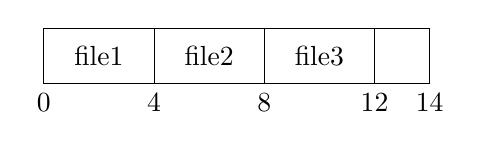
\begin{tikzpicture}[scale=.035]
\draw (0,0) rectangle (40,20);
\draw (40,0) rectangle (80,20);
\draw (80,0) rectangle (120,20);
\draw (120,0) rectangle (140,20);
\draw (20,10) node{file1};
\draw (60,10) node{file2};
\draw (100,10) node{file3};
\draw (0,-7) node{0};
\draw (40,-7) node{4};
\draw (80,-7) node{8};
\draw (120,-7) node{12};
\draw (140,-7) node{14};
\end{tikzpicture}\]
\iffalse
\[\begin{graph}(150,32)(-3,-12)
\graphlinecolour{0}
\fillednodesfalse
\rectnode{a}[40,20](20,10)
\rectnode{b}[40,20](60,10)
\rectnode{c}[40,20](100,10)
\rectnode{d}[20,20](130,10)
\autonodetext{a}{file1}
\autonodetext{b}{file2}
\autonodetext{c}{file3}
\freetext(0,-7){0}
\freetext(40,-7){4}
\freetext(80,-7){8}
\freetext(120,-7){12}
\freetext(140,-7){14}
\end{graph}\]
\fi
Suppose file2 is now deleted, resulting in a four-block gap, with
another two blocks free at the end of the disk:
\[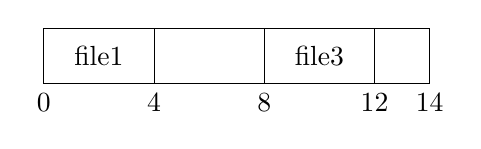
\begin{tikzpicture}[scale=.035]
\draw (0,0) rectangle (40,20);
\draw (40,0) rectangle (80,20);
\draw (80,0) rectangle (120,20);
\draw (120,0) rectangle (140,20);
\draw (20,10) node{file1};
\draw (100,10) node{file3};
\draw (0,-7) node{0};
\draw (40,-7) node{4};
\draw (80,-7) node{8};
\draw (120,-7) node{12};
\draw (140,-7) node{14};
\end{tikzpicture}\]
\iffalse
\[\begin{graph}(150,32)(-3,-12)
\graphlinecolour{0}
\fillednodesfalse
\rectnode{a}[40,20](20,10)
\rectnode{b}[40,20](60,10)
\rectnode{c}[40,20](100,10)
\rectnode{d}[20,20](130,10)
\autonodetext{a}{file1}
\autonodetext{c}{file3}
\freetext(0,-7){0}
\freetext(40,-7){4}
\freetext(80,-7){8}
\freetext(120,-7){12}
\freetext(140,-7){14}
\end{graph}\]
\fi
If, at this point, a three-block file (file4) is created, it can go
into the four-block gap, leaving one block unused:
\[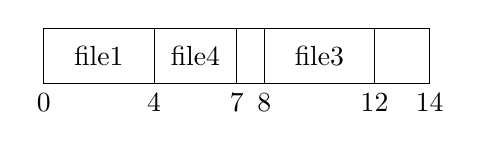
\begin{tikzpicture}[scale=.035]
\draw (0,0) rectangle (40,20);
\draw (40,0) rectangle (70,20);
\draw (70,0) rectangle (80,20);
\draw (80,0) rectangle (120,20);
\draw (120,0) rectangle (140,20);
\draw (20,10) node{file1};
\draw (100,10) node{file3};
\draw (55,10) node{file4};
\draw (0,-7) node{0};
\draw (40,-7) node{4};
\draw (70,-7) node{7};
\draw (80,-7) node{8};
\draw (120,-7) node{12};
\draw (140,-7) node{14};
\end{tikzpicture}\]
\iffalse
\[\begin{graph}(150,32)(-3,-12)
\graphlinecolour{0}
\fillednodesfalse
\rectnode{a}[40,20](20,10)
\rectnode{b}[30,20](55,10)
\rectnode{e}[10,20](75,10)
\rectnode{c}[40,20](100,10)
\rectnode{d}[20,20](130,10)
\autonodetext{a}{file1}
\autonodetext{c}{file3}
\autonodetext{b}{file4}
\freetext(0,-7){0}
\freetext(40,-7){4}
\freetext(70,-7){7}
\freetext(80,-7){8}
\freetext(120,-7){12}
\freetext(140,-7){14}
\end{graph}\]
\fi
Now there are three unused blocks, but there is no way to
satisfy another three-block allocation request, because the three
unused blocks are broken up, with one block between files 4 and 3, and
two more blocks at the end of the disk.

Notice that you wound up with a one-block gap not because a one-block
file was created and later deleted (or because of stupid allocation),
but because a four-block file was replaced by a three-block file.  The
resulting gap is the difference in the file sizes.  This means that
even if a disk is used exclusively for storing large files, it may
still wind up with small gaps, which cannot hold any large files.
This is the fundamental problem of external fragmentation.

Returning to the parallel parking analogy, consider an area where no
parking spaces are marked on the pavement, leaving drivers to allocate
their own spaces.  Even if they are courteous enough not to leave any
pointless gaps, small gaps will arise as cars of varying sizes come
and go.  A large car may vacate a space, which is then taken by a
smaller car.  The result is a gap equal to the difference in car
sizes, too small for even the smallest cars to use.  If this situation
happens repeatedly at different spots along a block, there may be enough
total wasted space to accommodate a car, but not all in one place.

Earlier, I mentioned that increasing the file system block size,
which increases internal fragmentation, decreases external
fragmentation.  The reason for this is that with a larger block size,
there is less variability in the amount of space being allocated.
Files that might have different sizes when rounded up to the next
kilobyte (say, 14~KB and 15~KB) may have the same size when rounded to
the next multiple of 4~KB (in this case, 16~KB and 16~KB).  Reduced
variability reduces external fragmentation; in the extreme case, no
external fragmentation at all occurs if the files are all allocated
the same amount of space.

Suppose you relax the requirement that a file be allocated a single
extent of the disk.  Using file metadata, it is possible to
store different blocks of the file in different locations, much as a
virtual memory address space can be scattered throughout physical
memory.  Does this mean that external fragmentation is a nonissue?
No, because for performance reasons, you will still want to allocate
the file contiguously as much as possible.  Therefore, external
fragmentation will simply change from being a space-efficiency issue
(free space that cannot be used) to a time-efficiency issue (free
space that cannot be used without file access becoming slower).  This
gets us into the next topic, locality.

\subsection{Locality}\label{locality-section}

Recall that disks provide their fastest performance when asked to
access a large number of consecutive sectors in a single request at a
location nearby to the previous access request. Most file system
designers have interpreted these conditions for fast access as implying the following
locality guidelines for space allocation:
\begin{enumerate}
\item The space allocated for each file should be broken into as few
extents as possible.
\item If a file needs to be allocated more than one extent, each
extent should be nearby to the previous one.
\item Files that are commonly used in close succession (or
concurrently) should be placed near one another.
\end{enumerate}

The connection between fast access and these three guidelines is
based on an implicit assumption that the computer system's
workload largely consists of accessing one file at a time and reading
or writing each file in its entirety, from beginning to end.  In some
cases, this is a reasonable approximation to the truth, and so the
preceding locality guidelines do result in good performance.
However, it is important to remember that the guidelines incorporate
an assumption about the workload as well as the disk performance
characteristics.  For some workloads, a different allocation strategy
may be appropriate.  In particular, as computing workloads are
consolidated onto a smaller number of computers
(using techniques such as virtualization, as discussed in Section~\ref{virtual-machines-subsection}),
file accesses become more jumbled.

As an example of a different allocation strategy that might make
sense, Rosenblum and Ousterhout suggested that blocks should be
allocated space on disk in the order they are written, without regard
to what files they belong to or what positions they occupy within
those files.  By issuing a large number of consecutive writes to the
disk in a single operation, this allows top performance for writing.
Even if the application software is concurrently writing to multiple files, and
doing so at random positions within those files, the write operations
issued to disk will be optimal, unlike with the more conventional file
layout.  Of course, read accesses will be efficient only if they are
performed in the same order as the writes were.  Fortunately, some
workloads do perform reads in the same order as writes, and some other
workloads do not need efficient read access.  In particular, the
efficiency of read access is not critical in a workload that reads most disk blocks
either never or repeatedly.  Those blocks that are never read are not a
problem, and those that are read repeatedly need only suffer the cost
of disk access time once and can thereafter be kept in RAM.

Returning to the more mainstream strategy listed at the beginning of
this subsection, the primary open question is how to identify files
that are likely to be accessed contemporaneously, so as to place them
nearby to one another on disk.  One approach, used in UNIX file
systems, is to assume that files are commonly accessed in conjunction
with their parent directory or with other (sibling) files in the same
directory.  Another approach is to not base the file placement on
assumptions, but rather on observed behavior.  (One assumption
remains: that future behavior will be like past behavior.)  For
example, Microsoft introduced a feature into Windows with the XP
version, in which the system observes the order of file accesses at
system boot time and also at application startup time, and then
reorganizes the disk space allocation based on those observed access
orders.  Mac OS~X does something similar as of version 10.3: it
measures which files are heavily used and groups them together.

\subsection{Allocation Policies and Mechanisms}
\label{fs-allocation}

Having seen the considerations influencing disk space allocation
(fragmentation and locality), you are now in a better position to
appreciate the specific allocation mechanism used by any particular
file system and the policy choices embodied in that mechanism.  The
full range of alternatives found in different file systems is too
broad to consider in any detail here, but I will sketch some
representative options.

Each file system has some way of keeping track of which disk blocks
are in use and which are free to be allocated.  The most common
representation for this information is a \vocab{bitmap}, that is, an
array of bits, one per disk block, with bit $i$
indicating whether block $i$ is in use.  With a bitmap, it is easy to
look for space in one particular region of the disk, but slow to
search an entire large disk for a desired size extent of free space.

Many UNIX and Linux file systems use a slight variant on the bitmap
approach.  Linux's ext3fs file system can serve as an example.  The
overall disk space is divided into modest-sized chunks known as
\vocabs{block group}.  On a system with 4-KB disk blocks,
a block group might encompass 128~MB.  Each block group has its own
bitmap, indicating which blocks within that group are free.  (In
Exercise~\ref{block-group-bitmap-exercise}, you can show that in the example given, each block group's
bitmap fits within a single block.)  Summary information for the file
system as a whole indicates how much free space each block group has,
but not the specific location of the free space within the block
groups.  Thus, allocation can be done in two steps: first find a
suitable block group using the summary information, and then find a
suitable collection of blocks within the block group, using its
bitmap.

I remarked earlier that UNIX and Linux file systems generally try to
allocate each file near its parent directory.  In particular, regular
files are placed in the same block group as the parent directory,
provided that there is any space in that group.  If this rule were
also followed for subdirectories, the result would be an attempt to
cram the entire file system into one block group.  Therefore, these
file systems use an alternative rule to choose a block group for a
subdirectory.

When creating a subdirectory, early versions of ext3fs and similar
file systems selected a
block group containing a lot of free space.
This spread the directories, with their corresponding files,
relatively evenly through the whole disk.  Because each new directory
went into a block group with lots of free space, there was a good
chance that the files contained in that directory would fit in the
same block group with it.  However, traversing a directory tree could
take a long time with these allocation policies, because each
directory might be nowhere near its parent directory.

Therefore, more recent versions of ext3fs and similar file systems
have used a different allocation policy for directories, developed by
Orlov.  A subdirectory is allocated in the parent directory's block
group, provided that it doesn't get too crowded.  Failing that, the
allocation policy looks through the subsequent block groups for one
that isn't too crowded.  This preserves locality across entire
directory trees without stuffing any block group so full of
directories that the corresponding files won't fit. The result can be
significant performance improvements for workloads that traverse
directory trees.

Once a file system decides to locate a file within a particular block
group, it still needs to allocate one or more extents of disk blocks
to hold the file's data.  (Hopefully those extents will all lie within
the chosen block group, although there needs to be a way for large
files to escape from the confines of a single block group.)

The biggest challenge in allocating extents is knowing how big an
extent to allocate.  Some older file systems required application
programmers to specify each file's size at the time the file was
created, so that the system could allocate an extent of corresponding
size.  However, modern systems don't work this way; instead, each file
grows automatically to accommodate the data written into it.

To meet this challenge, modern operating systems use a technique known
as \foldvocab{delayed}{allocation}.  As background, you need to
understand that operating systems do not normally write data to disk
the moment an application program issues a write request.  Instead,
the data is stored in RAM and written back to disk later.  This delay
in writing yields two options for when the disk space is allocated:
when the data goes into RAM or later when it gets written to disk.

Without delayed allocation, the operating system needs to choose a
disk block to hold the data at the time it goes into RAM.  The system
tags the data in RAM with the disk block in which that data belongs.  Later,
the system writes the data out to the specified location on disk.
This approach is simple, but requires the operating system to allocate
space for the first block of data as soon as it is generated, before
there is any clue how many more blocks will follow.

Delayed allocation puts off the choice of disk block until the time of
actually writing to disk; the data stored in RAM is tagged only with
the file it should be written to and the position within that file.
Now the operating system does not need to guess how much data a
program is going to write at the time when it generates the first
block.  Instead, it can wait and see how much data gets written and
allocate an extent that size.

Once the operating system knows the desired extent size, it needs to
search the data structure that records the available space.  Bitmaps
(whether in individual block groups or otherwise) are not the only
option for tracking free space.  The XFS file system, which was
particularly designed for large file systems, takes an alternative
approach.  It uses balanced search trees, known as
B-trees, to track the free extents of disk space.  One B-tree
stores the free extents indexed by their location while another
indexes them by their size.  That way, XFS can quickly locate free
space near a specified location on disk or can quickly locate a
desired amount of space.  Technically, the trees used by XFS are a
slight variant of B-trees, known as
B${}^+$-trees.  I'll describe this data
structure in Section~\ref{B-trees}.

With free extents indexed by size in a B${}^+$-tree, the XFS allocator can
naturally use a \vocab{best-fit} policy, where it finds the smallest
free extent bigger than the desired size.  (If the fit is not exact,
the extra space can be broken off and left as a smaller free extent.)
With a bitmap, on the other hand, the most natural allocation policy
is \vocab{first-fit}, the policy of finding the first free extent that is
large enough.  Each policy has its merits; you can compare them in
Exercise~\ref{best-fit-first-fit-exercise}.

\section{Metadata}\label{metadata-section}

You have seen that a file system is analogous to a virtual memory
system.  Each has an allocation policy to select concrete storage
locations for each chunk of data.  Continuing the analogy, I will now
explain the \vocab{metadata} that serves as the analog of page tables.  Recall that in a system with
separate address spaces, each process has its own page table, storing
the information regarding which page frame holds that process's page~0,
page~1, and so forth.  Similarly, each file has its
own metadata storing the information regarding which disk block holds
that file's block~0, block~1, and so forth.  You will see that, as with page
tables, there are several choices for the data structure holding this
mapping information.  I discuss these alternative structures in
Section~\ref{data-location-metadata-section}.

Metadata is data about data.  Information regarding where on disk the
data is stored is one very important kind of metadata.  However, I
will also more briefly enumerate other kinds.
First, in Section~\ref{access-control-metadata-section}, I will
revisit access control, a topic I considered
from another perspective in Chapter~\ref{processes-chapter}.  In Section~\ref{access-control-metadata-section}, the question
is not how access control information is enforced during access
attempts, but how it is stored in the file system.  Second, I will
look in Section~\ref{other-metadata-section} at the other more minor, miscellaneous kinds of metadata (beyond
data location and access control), such as access dates and times.

Some authors include file names as a kind of metadata.  This makes
sense in those file systems where each file has exactly one name.
However, most modern file systems do not fit this description; a file
might have no names, or might have multiple names.  Thus, you are
better off thinking of a name not as a property of a file, but as a
route that can lead to a file.  Similarly, in other persistence
services, data may be accessed through multiple routes, such as
database indexes.  Therefore, I will not include naming in this
section on metadata, instead including it in Section~\ref{directory-indexing-section} on
directories and indexing.

\subsection{Data Location Metadata}\label{data-location-metadata-section}

The simplest representation for data location metadata would be an
array of disk block numbers, with element $i$ of the array specifying
which disk block holds block $i$ of the file.  This would be analogous
to a linear page table.  Traditional UNIX file systems (including
Linux's ext2fs and ext3fs) use this approach for small files.  Each file's
array of disk block numbers is stored in the file's metadata structure
known as its \vocab{inode} (short for
\foldvocab{index}{node}).  For larger files, these file systems keep
the inodes compact by using indirect blocks, roughly
analogous to multilevel page tables.  I discuss the traditional form
of inodes and indirect blocks next.  Thereafter, I discuss two
alternatives used in some more modern file systems: extent maps, which
avoid storing information about individual blocks, and B${}^+$-trees, which
provide efficient access to large extent maps.

\subsubsection{Inodes and Indirect Blocks}

When UNIX was first developed in the early 1970s, one of its many
innovative features was the file system design, a design that has served as the
model for commonly used UNIX and Linux file systems to the present
day, including Linux's ext3fs.  The data-location metadata in these
systems is stored in a data structure that can better be called
expedient than elegant.  However, the structure is efficient for small files,
allows files to grow large, and can be manipulated by simple code.

Each file is represented by a compact chunk of data called an inode.
The inode contains the file's metadata if the file is small or an
initial portion of the metadata if the file is large.  By allowing
large files to have more metadata elsewhere (in indirect blocks), the
inodes are kept to a small fixed size.  Each file system contains an
array of inodes, stored in disk blocks set aside for the purpose,
with multiple inodes per block.  Each inode is identified by its position
in the array.  These inode numbers (or \vocabs{inumber}) are the
fundamental identifiers of the files in a file system; essentially, the
files are identified as
file~0, file~1, and so forth, which indicate the files with inodes in position 0,
1, and so forth.  Later, in Section~\ref{directory-indexing-section}, you'll see
how file names are mapped into inode numbers.

Each inode provides the metadata for one file.  The metadata includes the disk block numbers
holding that file's data, as well as the access permissions and other
metadata.  These categories of metadata are shown in Figure~\ref{initial-inode}.
\begin{figure}
\centerline{\begin{tabular}{|c|}
\hline
file block 0's disk block number\\\hline
file block 1's disk block number\\\hline
file block 2's disk block number\\\hline
$\vdots$\\\hline
access permissions\\\hline
other metadata\\\hline
\end{tabular}}
\caption{This initial approximation of an inode shows the principle
categories of metadata.   However, this diagram is unrealistic in that the list
of disk block numbers seems to be unlimited, whereas actual inodes
have only a limited amount of space.}
\label{initial-inode}
\end{figure}
In this simplified diagram, the inode directly contains the mapping
information specifying which disk block contains each block of the
file, much like a linear page table.  Recall, however, that inodes are
a small, fixed size, whereas files can grow to be many blocks long.
To resolve this conflict, each inode directly contains the mapping
information only for the first dozen or so blocks.  (The exact number
varies between file systems, but is consistent within any one file
system.)  Thus, a more realistic inode picture is as shown in
Figure~\ref{limited-inode}.
\begin{figure}
\centerline{\begin{tabular}{|c|}
\hline
file block 0's disk block number\\\hline
$\vdots$\\\hline
file block 11's disk block number\\\hline
indirect access to file block 12 through the end of the file\\\hline
access permissions\\\hline
other metadata\\\hline
\end{tabular}}
\caption{In this limited-size inode, blocks from number~12 to the end of the
file are indirectly referenced.}
\label{limited-inode}
\end{figure}

Before I go into detail on how further disk blocks are indirectly
accessed, I should emphasize one aspect of the inode design.  The
low-numbered blocks of a file are mapped in the exact same way
(directly in the inode) regardless of whether they are the only blocks
in a small file or the first blocks of a large file.  This means that
large files have a peculiar asymmetry, with some blocks more
efficiently accessible than others.  The advantage is that when a file
grows and transitions from being a small file to being a large one, the
early blocks' mapping information remains unchanged.

Because most files are small, the inodes are kept small, a fraction of
a block in size.  (If inodes were full blocks, the overhead for
single-block files would be 100 percent.)  For those files large enough to
overflow an inode, however, one can be less stingy in allocating space
for metadata.  Therefore, if the system needs more metadata space, it doesn't
allocate a second inode; it allocates a whole additional disk block, an
\foldvocab{indirect}{block}.  This provides room for many more
block numbers, as shown in Figure~\ref{single-indirect-inode}.  The
exact number of additional block numbers depends on how big blocks and
block numbers are.  With 4-KB blocks and 4-byte block numbers, an
indirect block could hold 1~K block numbers (that is, 1024 block
numbers), as shown in the figure.  This kind of indirect block is more
specifically called a \foldvocab{single}{indirect block}, because it
adds only a single layer of indirection: the inode points to it, and
it points to data blocks.
\begin{figure}
\centerline{\begin{tabular}{|c|c|c|}
\multicolumn{1}{c}{\textbf{Inode}}&\multicolumn{1}{c}{\hspace{1em}}&\multicolumn{1}{c}{\textbf{Indirect block}}\\\cline{1-1}\cline{3-3}
file block 0's disk block number&&file block 12's disk block number\\\cline{1-1}\cline{3-3}
$\vdots$&&$\vdots$\\\cline{1-1}\cline{3-3}
file block 11's disk block number&&file block 1035's disk block number\\\cline{1-1}\cline{3-3}
indirect block's block number&\multicolumn{1}{c}{}&\multicolumn{1}{c}{}\\\cline{1-1}
access permissions&\multicolumn{1}{c}{}&\multicolumn{1}{c}{}\\\cline{1-1}
other metadata&\multicolumn{1}{c}{}&\multicolumn{1}{c}{}\\\cline{1-1}
\end{tabular}}
\caption{If an inode were used with a single indirect block, the block
numbers would be stored as shown here. Note that the indirect
block is actually considerably larger than the inode, contrary to its
appearance in the figure.}
\label{single-indirect-inode}
\end{figure}

In this example with 4-KB blocks, the single indirect block allows you
to accommodate files slightly more than 4~MB in size.  To handle
yet-larger files, you can use a multilevel tree scheme, analogous to
multilevel page tables.  The inode can contain a block number for a
double indirect block, which contains block numbers for many more
single indirect blocks, each of which contains many data block
numbers.  Figure~\ref{double-indirect-inode} shows this enhancement to
the inode design, which retains the dozen direct blocks and the original single
indirect block, while adding a double indirect block.
\begin{figure}
\centerline{\begin{tabular}{|c|c|c|}
\multicolumn{1}{c}{\textbf{Inode}}&\multicolumn{1}{c}{\hspace{1em}}&\multicolumn{1}{c}{\textbf{Single
indirect block}}\\\cline{1-1}\cline{3-3}
file block 0's disk block number&&file block 12's disk block number\\\cline{1-1}\cline{3-3}
$\vdots$&&$\vdots$\\\cline{1-1}\cline{3-3}
file block 11's disk block number&&file block 1035's disk block number\\\cline{1-1}\cline{3-3}
single indirect block's number&\multicolumn{1}{c}{}&\multicolumn{1}{c}{}\\\cline{1-1}
double indirect block's number&\multicolumn{1}{c}{}&\multicolumn{1}{c}{}\\\cline{1-1}
access permissions&\multicolumn{1}{c}{}&\multicolumn{1}{c}{}\\\cline{1-1}
other metadata&\multicolumn{1}{c}{}&\multicolumn{1}{c}{}\\\cline{1-1}
\end{tabular}}
\vspace*{1em}
\centerline{\begin{tabular}{|c|c|c|}
\multicolumn{1}{c}{\textbf{Double indirect
block}}&\multicolumn{1}{c}{\hspace{1em}}&\multicolumn{1}{c}{\textbf{Indirect
block 1}}\\\cline{1-1}\cline{3-3}
indirect block 1's block number&&file block 1036's disk block number\\\cline{1-1}\cline{3-3}
$\vdots$&&$\vdots$\\\cline{1-1}\cline{3-3}
indirect block 1024's block number&&file block 2059's disk block number\\\cline{1-1}\cline{3-3}
\end{tabular}}
\vspace*{1em}
\textbf{Indirect blocks 2--1024:} similar to indirect block 1
\caption{If an inode were used with single and double indirect blocks,
the block numbers would be stored as shown here.}
\label{double-indirect-inode}
\end{figure}

Because the double indirect block points at many indirect blocks, each
of which points at many data blocks, files can now grow quite large.
(In Exercise~\ref{largest-double-indirect-exercise}, you can figure out just how large.)  However, many
UNIX file systems go one step further by allowing the inode to point
to a triple indirect block as well, as shown in
Figure~\ref{inode-block-tree}.  Comparing this with multilevel page
tables is illuminating; the very unbalanced tree used here allows a
small, shallow tree to grow into a large, deeper tree in a
straightforward way.  Later you'll see that B${}^+$-trees grow somewhat less
straightforwardly, but without becoming so imbalanced.
\begin{figure}
\centerline{\includegraphics{hail_f0810}}
\iffalse
\centerline{\begin{graph}(417,140)(8,355)
\graphnodesize{0}
\graphnodecolour{1}
\grapharrowlength{5}
\textnode{inode}(200, 490){inode}[\graphlinewidth{0}\graphlinecolour{1}]
\textnode{directl}(20, 465){}[\graphlinewidth{0}\graphlinecolour{1}]
\freetext(91,472){\ldots}
\textnode{directr}(80, 465){}[\graphlinewidth{0}\graphlinecolour{1}]
\textnode{direct}(50, 460){a few data blocks}[\graphlinewidth{0}\graphlinecolour{1}]
\textnode{single}(142, 460){single indirect}[\graphlinewidth{0}\graphlinecolour{1}]
\textnode{double}(244, 460){double indirect}[\graphlinewidth{0}\graphlinecolour{1}]
\textnode{triple}(346, 460){triple indirect}[\graphlinewidth{0}\graphlinecolour{1}]
\textnode{sdatal}(112, 435){}[\graphlinewidth{0}\graphlinecolour{1}]
\freetext(142,445){\ldots}
\textnode{sdatar}(172, 435){}[\graphlinewidth{0}\graphlinecolour{1}]
\textnode{sdata}(142, 430){many data blocks}[\graphlinewidth{0}\graphlinecolour{1}]
\textnode{dsinglel}(214, 435){}[\graphlinewidth{0}\graphlinecolour{1}]
\freetext(244,445){\ldots}
\textnode{dsingler}(274, 435){}[\graphlinewidth{0}\graphlinecolour{1}]
\textnode{dsingle}(244, 430){many indirect blocks}[\graphlinewidth{0}\graphlinecolour{1}]
\textnode{dsinglelb}(214, 425){}[\graphlinewidth{0}\graphlinecolour{1}]
\textnode{dsinglerb}(274, 425){}[\graphlinewidth{0}\graphlinecolour{1}]
\textnode{dsdatall}(204, 405){}[\graphlinewidth{0}\graphlinecolour{1}]
\freetext(217,413){\ldots}
\textnode{dsdatalr}(234, 405){}[\graphlinewidth{0}\graphlinecolour{1}]
\freetext(244,417){\ldots}
\textnode{dsdatarl}(254, 405){}[\graphlinewidth{0}\graphlinecolour{1}]
\freetext(271,413){\ldots}
\textnode{dsdatarr}(284, 405){}[\graphlinewidth{0}\graphlinecolour{1}]
\textnode{dsdata}(244, 400){tons of data blocks}[\graphlinewidth{0}\graphlinecolour{1}]
\textnode{tdoublel}(316, 435){}[\graphlinewidth{0}\graphlinecolour{1}]
\freetext(346,445){\ldots}
\textnode{tdoubler}(376, 435){}[\graphlinewidth{0}\graphlinecolour{1}]
\textnode{tdouble}(346, 430){many double}[\graphlinewidth{0}\graphlinecolour{1}]
\textnode{tdoubleb}(346, 420){indirect blocks}[\graphlinewidth{0}\graphlinecolour{1}]
\textnode{tdoublelb}(316, 415){}[\graphlinewidth{0}\graphlinecolour{1}]
\textnode{tdoublerb}(376, 415){}[\graphlinewidth{0}\graphlinecolour{1}]
\textnode{tdsinglell}(306, 395){}[\graphlinewidth{0}\graphlinecolour{1}]
\freetext(319,403){\ldots}
\textnode{tdsinglelr}(336, 395){}[\graphlinewidth{0}\graphlinecolour{1}]
\freetext(346,407){\ldots}
\textnode{tdsinglerl}(356, 395){}[\graphlinewidth{0}\graphlinecolour{1}]
\freetext(373,403){\ldots}
\textnode{tdsinglerr}(386, 395){}[\graphlinewidth{0}\graphlinecolour{1}]
\textnode{tdsingle}(346, 390){tons of indirect blocks}[\graphlinewidth{0}\graphlinecolour{1}]
\textnode{tdsinglelb}(316, 385){}[\graphlinewidth{0}\graphlinecolour{1}]
\textnode{tdsinglerb}(376, 385){}[\graphlinewidth{0}\graphlinecolour{1}]
\textnode{tdsdatall}(306, 365){}[\graphlinewidth{0}\graphlinecolour{1}]
\freetext(319,373){\ldots}
\textnode{tdsdatalr}(336, 365){}[\graphlinewidth{0}\graphlinecolour{1}]
\freetext(346,377){\ldots}
\textnode{tdsdatarl}(356, 365){}[\graphlinewidth{0}\graphlinecolour{1}]
\freetext(373,373){\ldots}
\textnode{tdsdatarr}(386, 365){}[\graphlinewidth{0}\graphlinecolour{1}]
\textnode{tdsdata}(346, 360){astronomically many data blocks}[\graphlinewidth{0}\graphlinecolour{1}]
\diredge{inode}{directl}
\diredge{inode}{directr}
\diredge{inode}{single}
\diredge{inode}{double}
\diredge{inode}{triple}
\diredge{single}{sdatal}
\diredge{single}{sdatar}
\diredge{double}{dsinglel}
\diredge{double}{dsingler}
\diredge{dsinglelb}{dsdatall}
\diredge{dsinglelb}{dsdatalr}
\diredge{dsinglerb}{dsdatarl}
\diredge{dsinglerb}{dsdatarr}
\diredge{triple}{tdoublel}
\diredge{triple}{tdoubler}
\diredge{tdoublelb}{tdsinglell}
\diredge{tdoublelb}{tdsinglelr}
\diredge{tdoublerb}{tdsinglerl}
\diredge{tdoublerb}{tdsinglerr}
\diredge{tdsinglelb}{tdsdatall}
\diredge{tdsinglelb}{tdsdatalr}
\diredge{tdsinglerb}{tdsdatarl}
\diredge{tdsinglerb}{tdsdatarr}
\end{graph}}
\fi
\caption{The full structure of a file starts with an inode and
continues through a tree of single, double, and triple indirect
blocks, eventually reaching each of the data blocks.}
\label{inode-block-tree}
\end{figure}

Having presented this method of mapping file blocks into disk blocks, I
will shortly turn to an alternative that avoids storing information on
a per-block basis.  First, however, it is worth drawing one more
analogy with page tables.  Just as a page table need not provide a
page frame number for every page (if some pages are not in memory), an
inode or indirect block need not provide a disk block number for every
block of the file.  Some entries can be left blank, typically by using
some reserved value that cannot be mistaken for a legal disk block
number.  This is valuable for \foldvocabs{sparse}{file}, also known as
files with \vocabs{hole}.  A sparse file has one or more large
portions containing nothing but zeros, usually because those portions
have never been written.  By not allocating disk blocks for the
all-zero file blocks, the file system can avoid wasting space and time.

\subsubsection{Extent Maps}

You have seen that traditional inodes and indirect blocks are based
around the notion of a \foldvocab{block}{map}, that is, an array
specifying a disk block number for each file block.  A block map is
completely general, in that each file block can be mapped to any disk
block.  File block $n$ can be mapped somewhere totally different on
disk from file block $n-1$.  Recall, however, that file system designers prefer
not to make use of this full generality.  For performance reasons,
consecutive file blocks will normally be allocated consecutive disk
blocks, forming long extents.  This provides the key to a more
efficient data structure for storing the mapping information.

Suppose you have a file that is 70 blocks long and that occupies
disk blocks 1000--1039 and 1200--1229.  A
block map would contain each one of those 70 disk block numbers.  An
\foldvocab{extent}{map}, on the other hand, would contain only two
entries, one for each of the file's extents, just as the opening
sentence of this paragraph contains two
ranges of block numbers.  Each entry in the extent
map needs to contain enough information to describe one extent.  There
are two alternatives for how this can be done:
\begin{itemize}
\item
Each entry can contain the extent's length and starting disk block
number.  In the example, the two extent map entries would be $(40,
1000)$ and $(30, 1200)$.  These say the file contains 40 blocks
starting at disk block 1000 and 30 blocks starting at disk block
1200.
\item
Each entry can contain the extent's length, starting file block
number, and starting disk block number.  In the example, the two
extent map entries would be $(40, 0, 1000)$ and $(30, 40, 1200)$.  The
first entry describes an extent of 40 blocks, starting at position 0 in the
file and occupying disk blocks starting with number 1000.  The second entry
describes an extent of 30 blocks, starting
at position 40 in the file and occupying disk blocks starting with number 1200.
\end{itemize}
The first approach is more compact.  The second approach, however, has the
advantage that each extent map entry can be understood in isolation,
without needing to read the preceding extent map entries.  This is
particularly useful if the extent map is stored in a B${}^+$-tree, as I
will discuss subsequently. For simplicity, I will assume the second approach
in the remainder of my discussion, though there are systems that use
each.

At first, it may not be obvious why extent maps are a big improvement.
A typical block map system might use a 4-byte block number to refer
to each 4-KB block.  This is less than one-tenth of one percent space
overhead, surely affordable with today's cheap disk storage.  What
reason do file system designers have to try to further reduce such an already small
overhead?  (I will ignore the possibility that the extent map takes
more space than the block map, which would happen only if the file is
scattered into lots of tiny extents.)

The key fact is that disk space efficiency turns into time efficiency,
which is a much more precious commodity.  Indirect blocks result in
extra disk I/O operations.  Consider, for example, reading a file that
is stored in a single 20-block extent.  With the block map
approach, the file system would need to do at least two disk read
operations: one to read the single indirect block and one to read the
data blocks.  This assumes the inode is already cached in memory,
having been read in along with other inodes in its disk block, and
that the file system is smart enough to read all 20 data blocks in
a single operation.  With an extent map, the entire mapping
information would fit in the inode; if you again assume the inode is
cached, a single read operation suffices.  Thus, the system can read
files like this twice as fast.  Admittedly, this is a somewhat
artificial best-case example.  However, even with realistic workloads,
a significant speedup is possible.

Several modern file systems use extent maps, including Microsoft
Windows' NTFS, Mac OS~X's HFS Plus, and XFS, which was ported into
Linux from SGI's IRIX version of UNIX.  For files that have only a
handful of extents (by far the most common case), all three store the
sequence of extent map entries in the inode or (in Windows and Mac
OS~X) in the corresponding inode-like structure.  The analogs of inodes in
NTFS are large enough (1~KB) that they can directly store entire
extent maps for most files, even those with more than a few extents. The other
two file systems use smaller inodes (or inode-like structures) and so
provide an interesting comparison of techniques for handling the
situation where extra space is needed for a large extent map.

HFS Plus takes an approach quite reminiscent of traditional UNIX
inodes: the first eight extent map entries are stored directly in the
inode-like structure, whether they are the only ones or just the first
few of a larger number.  Any additional entries are stored elsewhere,
in a single B${}^+$-tree that serves for all the files, as I will describe
subsequently.  XFS, on the other hand, stores all the extent map entries for
a file in a file-specific B${}^+$-tree; the space in the inode is the root
node of that tree.  When the tree contains only a few extents, the
tree is small enough that the
root of the tree is also a leaf, and so the extents are directly in
the inode, just as with HFS Plus.  When the extent map grows larger,
however, all the entries move down into descendant nodes in the tree,
and none are left in the inode, unlike HFS Plus's special treatment of
the first eight.

\subsubsection{B-Trees}\label{B-trees}

The \vocab{B-tree} data structure is a balanced search tree structure
generally configured with large, high-degree nodes forming shallow,
bushy trees.  This property makes it well suited to disk storage,
where transferring a large block of data at once is efficient (hence,
large nodes), but performing a succession of operations is slow (hence,
a shallow tree).  You may have encountered B-trees before,
in which case my summary will be a review, with the exception
of my description of specific applications for which this structure
is used.

Any B-tree associates search keys with corresponding values, much like
a dictionary associates words with their definitions or a phone book
associates names with phone numbers.  The keys can be textual strings
organized in alphabetic order (as in these examples) or numbers
organized by increasing value; all that is required is that there is
some way to determine the relative order of two keys.

The B-tree allows entries to be efficiently located by key, as well as
inserted and deleted.  Thus far, the same could be said for a hash
table structure, such as is used for hashed page tables.  Where
B-trees (and other balanced search trees) distinguish themselves is
that they also provide efficient operations based on the ordering of
keys, rather than just equality of keys.  For example, if someone asks
you to look up ``Smit'' in a phone book, you could reply, ``There is no
Smit; the entries skip right from Smirnoff to Smith.''  You could do
the same with a B-tree, but not with a hash table.

This ability to search for neighbors of a key, which need not itself
be present in the tree, is crucial when B-trees are used for extent
maps.  Someone may want information about the extent containing file
block 17.  There may be no extent map entry explicitly mentioning 17;
instead, there is an entry specifying a 10-block extent starting with
file block 12.  This entry can be found as the one with the largest key
that is less than or equal to 17.

B-trees can play several different roles in persistence systems.  In
Section~\ref{directory-indexing-section}, you'll see their use for
directories of file names and for indexes of database contents; both
are user-visible data access services.  In the current section,
B-trees play a
more behind-the-scenes role, mapping positions within a file to
locations on disk.  Earlier, in Section~\ref{fs-allocation}, you saw
another related use, the management of free space for allocation.  The
data structure fundamentals are the same in all cases; I choose to
introduce them here, because extent maps seem like the simplest
application.  Free space mapping is complicated by the dual indexing
(by size and location), and directories are complicated by the use of
textual strings as keys.

You are probably already familiar with binary search trees, in which
each tree node contains a root key and two pointers to subtrees, one
with keys smaller than the root key, and one with keys larger than the
root key.  (Some convention is adopted for which subtree contains keys
equal to the root key.)  B-tree nodes are similar, but rather than
using a single root key to make a two-way distinction, they use $N$
root keys to make an $N+1$ way distinction.  That is, the root node
contains $N$ keys (in ascending order) and $N+1$ pointers to subtrees,
as shown in Figure~\ref{scan-8-1}.
\begin{figure}
\centerline{\includegraphics{hail_f0811}}
%\centerline{\def\epsfsize#1#2{0.6#1}\epsfbox{scan-8-1.eps}}
\caption{A B-tree node contains $N$ keys and $N+1$ pointers to the
subtrees under it.  Each subtree contains keys in a particular range.}
\label{scan-8-1}
\end{figure}
The first subtree contains keys smaller than the first root key, the
next subtree contains keys between the first and second root keys,
and so forth.  The last subtree contains keys larger than the last root key.

If a multi-kilobyte disk block is used to hold a B-tree node, the
value of $N$ can be quite large, resulting in a broad, shallow tree.
In fact, even if a disk block were only half full with root keys and
subtree pointers, it would still provide a substantial branching
factor.  This observation provides the inspiration for the mechanism
used to maintain B-trees as entries are inserted.

Each node is allowed to be anywhere between half full and totally
full.
This flexibility means one can easily insert into a node, so long as
it is less than full.
The hard case can be handled by
splitting nodes.  As a special exception, the root node is not
required to be even half full.  This exception allows you to build a
tree with any number of entries, and it adds at most one level to the height
of the tree.

Consider, for example, inserting one more entry into an already full
node.  After insertion, you have $N+1$ keys but only room for $N$.  The node
can be replaced with two nodes, one containing the $N/2$ smallest keys
and the other the $N/2$ largest keys.  Thus, you now have two half-full
nodes.  However, you have only accounted for $N$ of the $N+1$ keys; the
median key is still left over.  You can insert this median key into the
parent node, where it will serve as the divider between the two
half-full nodes, as shown in Figure~\ref{B-tree-split}.
\begin{figure}
\centerline{\includegraphics{hail_f0812}}
%\centerline{\def\epsfsize#1#2{0.6#1}\epsfbox{B-tree-split.eps}}
\caption{Inserting 16 into the illustrated B-tree, which has
node-capacity 4, causes a node to split, with the median key moving
into the parent.}
\label{B-tree-split}
\end{figure}

When you insert the median key into the parent node, what if the
parent node is also full?  You split the parent as well.  The splitting
process can continue up the tree, but because the tree is shallow, this
won't take very long.  If the node being split has no parent, because
it is the root of the tree, it gains a new parent holding just the
median key.  In this way the tree grows in height by one level.

In Bayer and McCreight's 1972 paper introducing B-trees, they
suggested that each node contain key/value pairs, along with pointers
to subtrees.  Practical applications today instead use a variant,
sometimes called \vocabindex{B${}^+$-trees}{B-tree}.  In a
B${}^+$-tree, the nonleaf nodes contain just keys and pointers to
subtrees, without the keys having any associated values.  The keys in
these nodes are used solely for navigation to a subtree.  The leaves
contain the key/value pairs that are the actual contents of the data
structure.  For example, a small B${}^+$-tree of extent map entries
might be organized as shown in Figure~\ref{B-plus-tree}.
\begin{figure}
\centerline{\includegraphics{hail_f0813}}
%\centerline{\def\epsfsize#1#2{0.6#1}\epsfbox{B-plus-tree.eps}}
\caption{This small B${}^+$-tree extent map contains information that
can be used to find
each extent's range of file block numbers and range of disk block
numbers.  Because the tree is a B${}^+$-tree rather than a B-tree, all
the extents are described in the leaves, with the nonleaf node containing
just navigational information.}
\label{B-plus-tree}
\end{figure}

This sort of B${}^+$-tree can store the extent map for a single file,
as is done in XFS.  For Mac OS~X's HFS Plus, a slightly different
approach is needed, because all files' extent maps are combined into a
single B${}^+$-tree.  (Recall, though, that the first eight extents of
each file are not included in this tree.)

Each entry in this file system's B${}^+$-tree describes an extent map
entry for some position within some file.  That is, the entry contains
a file number (analogous to an inode number), a starting block number
within the file, a length in blocks, and a starting disk block
number.  The concatenation of file number and starting file block
number serves as the key.  That way, all the entries for a particular
file appear consecutively in the tree, in order by their position
within the file.

The insertion algorithm for B${}^+$-trees is a slight variant of the
one for pure B-trees; you can work through the differences in
Exercise~\ref{Bplus-tree-insertion-exercise}.

\subsection{Access Control Metadata}\label{access-control-metadata-section}

The complexity of the data structures storing access control
information is directly related to the sophistication of the
protection system.  Recall that the POSIX specification, followed by
UNIX and Linux, provides for only fixed-length access control lists
(ACLs), with permissions for a file's owner, owning group, and
others.  This information can be stored compactly in the file's
inode.  Microsoft Windows, on the other hand, allows much more general
ACLs.  Thus, the designers of NTFS have faced a more interesting
challenge and, in fact, have revisited their design decision, as you
will see.

For POSIX-compliant access control, an inode can contain three
numbers: one identifying the file's owning user, one identifying the
file's owning group, and one containing nine bits, representing the
\verb|rwx| permissions for the owning user, the owning group, and other users.  This third
number, containing the nine permission bits, is called the file's
\vocab{mode}.  Rather than waste all but nine bits in the mode, the
others are used to encode additional information, such as whether the
file is a regular file, a directory, an I/O device, and so forth.
Figure~\ref{stater-source} shows how the permissions can be determined
by extracting an inode's mode using the {\tt stat} system call.  (This
system call differs only slightly from {\tt fstat}, which you saw
earlier.  The file is specified by name, rather than by a numerical
file descriptor.)  If you compile this C$++$ program and call the
resulting executable {\tt stater}, then a command like
\verb|./stater somefile| should produce information you could also get
with \verb|ls -l somefile|.
\begin{figure}
\begin{verbatim}
#include <unistd.h>
#include <time.h>
#include <sys/stat.h>
#include <stdio.h>
#include <iostream>
using namespace std;

static void print_bit(int test, char toPrint){
  if(test)
    cout << toPrint;
  else
    cout << '-';
}

int main(int argc, char *argv[]){
  if(argc != 2){
    cerr << "Usage: " << argv[0] << " filename" << endl;
    return -1;
  }
  struct stat info;
  if(stat(argv[1], &info) < 0){
    perror(argv[1]);
    return -1;
  }
  print_bit(info.st_mode & S_IRUSR, 'r');
  print_bit(info.st_mode & S_IWUSR, 'w');
  print_bit(info.st_mode & S_IXUSR, 'x');
  print_bit(info.st_mode & S_IRGRP, 'r');
  print_bit(info.st_mode & S_IWGRP, 'w');
  print_bit(info.st_mode & S_IXGRP, 'x');
  print_bit(info.st_mode & S_IROTH, 'r');
  print_bit(info.st_mode & S_IWOTH, 'w');
  print_bit(info.st_mode & S_IXOTH, 'x');
  cout << endl;
  return 0;
}
\end{verbatim}
\caption{This C$++$ program, {\tt stater.cpp}, uses {\tt stat} to
  retrieve access control metadata for whichever file is specified by
  the command-line argument {\tt argv[1]}.}
\label{stater-source}
\end{figure}

Early versions of NTFS stored the full ACL for each file
independently.  If the ACL was small enough to fit in the inode-like
structure, it was stored there.  Otherwise, it was stored in one or
more extents of disk blocks, just like the file's data, and the
inode-like structure contained an extent map for the ACL.

As of Windows 2000, Microsoft redesigned NTFS to take advantage of the
fact that many files have identical ACLs.  The contents of the ACLs are
now stored in a centralized database.  If two files have identical
ACLs, they can share the same underlying representation of that ACL.

\subsection{Other Metadata}\label{other-metadata-section}

Because files can be of any length, not just a multiple of the block
size, each inode (or equivalent) contains the file's size in bytes.
(The program in Figure~\ref{fstater-source} on page~\pageref{fstater-source} showed how you can
retrieve this information.)  Other metadata is much more
system-specific.  For example, POSIX specifies that each file has
three time stamps, recording when the file was last accessed, last
written, and last modified in any way. Modification includes not only  writing the
data, but also making changes in
permission and other metadata attributes.  NTFS records whether
the file should be hidden in ordinary directory listings.  HFS Plus
has many metadata attributes supporting the graphical user interface;
for example, each file records its icon's position.

One metadata attribute on POSIX systems connects with file linking,
that is, the use of multiple names for one file, which is the
topic of Section~\ref{file-linking-section}.  Each file's inode contains a count of how many names
refer to the file.  When that count reaches zero and the file is not
in use by any process, the operating system deletes the file.  The
operation users normally think of as deleting a file actually just
removes a name; the underlying file may or may not be deleted as a
consequence.

\section{Directories and Indexing}
\label{directory-indexing-section}

Having seen how file systems provide the storage for files, you are now ready to
consider how those
systems allow files to be located by name.  As a similar question regarding
database systems, you can consider how those systems provide indexed lookup.  In
Section~\ref{directory-index-comparison-section}, I set the stage for
this discussion by presenting a common framework for file directories
and database indexes, showing the ways in which they differ.
In Section~\ref{spotlight-section}, I show how the separation
between file directories and database indexes is currently weakening
with the introduction of indexing mechanisms for locating files.
Having shown the basic principles of both directories and indexes, I use
Section~\ref{file-linking-section} to dig into one particular aspect of
file directories in more detail: the ways in which multiple names can
refer to a single file.  Finally, in
Section~\ref{directory-index-structures-section}, I take you behind
the scenes to look at typical data structures used for directories and indexes.

\subsection{File Directories Versus Database Indexes}\label{directory-index-comparison-section}

Traditionally, file systems include \vocabyies{director}, which provide access
to files by name.  Databases, on the other hand, include \vocabes{index},
which provide access to entries in the database based on a portion of
the contents.  This clean distinction between file systems and
databases is currently blurring, as alternative file-access techniques
based on indexes become available.  In particular, Apple introduced
such a feature in Mac OS~X version 10.4 under the name Spotlight.  I
describe Spotlight in Section~\ref{spotlight-section}.  Microsoft
subsequently included a related feature in
Windows Vista.  This trend makes it even more
important to see what directories and indexes have in common and what
distinguishes them.

Both directories and indexes provide a mapping from keys to objects.
The keys in a directory are names, which are external to the object
being named.  You can change the contents of a file without changing
its name or change the name without changing the contents.  In
contrast, the keys in an index are attributes of the indexed objects,
and so are intrinsic to those objects.  For example, an index on a
database table of chapters might allow direct access to the row with
title {\tt "\persistenceChapterTitle"} or with the number {\tt
\ref{persistence-chapter}}.  If the row were updated to show a change
in this chapter's title or number, the index would need to be updated
accordingly.  Similarly, any update to the index must be in the context of
a corresponding change to
the indexed row; it makes no sense to say that you want
to look up the row under chapter number {\tt 1}, but there find that
the real chapter number is still {\tt \ref{persistence-chapter}}.

Each name in a directory identifies a single file.  Two files may have
the same name in different directories, but not in the same directory.
Database indexes, on the other hand, can be either for a unique
attribute or a non-unique one.  For example, it may be useful to index
a table of user accounts by both the unique login name and the
non-unique last name.  The unique index can be used to find the single
record of information about the user who logs in as {\tt "jdoe"},
whereas the non-unique index can be used to find all the records of
information about users with last name {\tt "Doe"}.    An index can
also use a combination of multiple attributes as its key.  For
example, a university course catalog could have a unique index
keyed on the combination of department and course number.

The final distinction between file directories and database indexes is
the least fundamental; it is the kind of object to which they provide
access.  Traditionally, directories provide access to entire files,
which would be the analog of tables in a relational database.
Indexes, on the other hand, provide access not to entire tables, but
rather to individual rows within those tables.  However, this
distinction is misleading for two reasons:
\begin{itemize}
\item
Database systems typically have a meta-table that serves as a catalog
of all the tables.  Each row in this meta-table describes one table.
Therefore, an index on this meta-table's rows is really an index of
the tables.  Access to its rows is used to provide access to the
database's tables.
\item
As I mentioned earlier, operating system developers are incorporating
indexes in order to provide content-based access to files.  This is
the topic of Section~\ref{spotlight-section}.
\end{itemize}

\subsection{Using Indexes to Locate Files}\label{spotlight-section}

As I have described, files are traditionally accessed by name, using
directories.  However, there has been considerable interest recently
in using indexes to help users locate files by content or other
attributes. Suppose that I could not remember the name
of the file containing this book.  That would not be a disaster, even
leaving aside the possibility that the world might be better off
without the book.  I could search for the file in numerous ways; for
example, it is one of the few files on my computer that has hundreds
of pages.  Because the Mac OS X system that I am using indexes files
by page count (as well as by many other attributes), I can simply ask for all
files with greater than 400 pages.  Once I am shown the five files
meeting this restriction, it is easy to recognize the one I am seeking.

The index-based search feature in Mac OS X, which is called Spotlight,
is not an integral component of the file system in the way directories
and filenames are.  Instead, the indexing and search are provided by
processes external to the operating system, which can be considered a
form of middleware.

The file system supports the indexing through a generic ability to
notify processes of events such as the creation or deletion of a file,
or a change in a file's contents.  These events can be sent to any
process that subscribes to them and are used for other purposes as
well, such as keeping the display of file icons up to date.  The
Spotlight feature uses it to determine when files need reindexing.
When I save out a new version of my book, the file system
notifies Spotlight that the file changed, allowing Spotlight to update
indexes such as the one based on page count.  Unlike file directories,
which are stored in a special data structure internal to the
file system, the indexes for access based on contents or attributes
like page counts are stored in normal files in the
\verb|/.Spotlight-V100| directory.

Apple refers to the indexed attributes (other than the actual file
contents) as metadata.  In my book example, the number of pages in a
document would be one piece of metadata.  This usage of the word
``metadata'' is rather different from its more traditional use in
file systems.  Every file has a fixed collection of file system metadata
attributes, such as owner, permissions, and time of last modification.
By contrast, the Spotlight metadata attributes are far more numerous,
and the list of attributes is open-ended and specific to
individual types of files.  For example, while the file containing my
book has an attribute specifying the page count, the file containing one of my
vacation photos has an attribute specifying the exposure time in
seconds.
Each attribute makes sense for the corresponding
file, but would not make sense for the other one.

As you have seen, the metadata attributes that need indexing are
specific to individual types of files.  Moreover, even common
attributes may need to be determined in different ways for different
types of files.  For example, reading a PDF file to determine its
number of pages is quite different from reading a Microsoft Word file
to determine its number of pages---the files are stored in totally
different formats.  Therefore, when the indexing portion of Spotlight
receives notification from the file system indicating that a file has
changed, and hence should be indexed, it delegates the actual indexing
work to a specialist indexing program that depends on the type of
file.  When you install a new application program on your system, the
installation package can include a matching indexing program.  That
way you will always be able to search for files on your system using
relevant attributes, but without Apple having had to foresee all the
different file types.

\subsection{File Linking}\label{file-linking-section}

Indexed attributes, such as page counts, are generally not unique.  My
system may well have several five-page documents.  By contrast, you have
already seen that each name within a directory names a single file.
Just because each pathname specifies a single file does not mean the
converse is true, however.  In this subsection, I will explain two
different ways in which a file can be reachable through multiple
names.

The most straightforward way in which multiple names can reach a
single file is if the directory entry for each of the names specifies
the same file.  Figure~\ref{hardlink} shows a directory with two
names, both referring to the same file.  In interpreting this figure, you should
understand that the box labeled as the file does not denote just the
data contained in the file, but also all of the file's metadata,
such as its permissions.
\begin{figure}
\centerline{\includegraphics{hail_f0815}}
%\centerline{\def\epsfsize#1#2{0.6#1}\epsfbox{hardlink.eps}}
\caption{A directory can contain two names for one file.}\label{hardlink}
\end{figure}
In the POSIX API, this
situation could have arisen in at least two different ways:
\begin{itemize}
\item
The file was created with the name \verb|alpha|, and then the
procedure call \verb|link("alpha", "beta")| added the name \verb|beta|.
\item
The file was created with the name \verb|beta|, and then the
procedure call \verb|link("beta", "alpha")| added the name \verb|alpha|.
\end{itemize}
No matter which name is the original and which is added, the two play
identical roles afterward, as shown in Figure~\ref{hardlink}.  Neither can be
distinguished as the ``real'' name.  Often people talk of the added
name as a \vocab{link} to the file.  However, you need to understand that \emph{all} file
names are links to files.  There is nothing to distinguish one added
with the \verb|link| procedure.

POSIX allows a file to have names in multiple directories, so long as all the directories are in the same file system.  In the
previous illustration (Figure~\ref{hardlink}),
\verb|alpha| and \verb|beta| in the current directory named one
file. Instead, I could have had directory entries in multiple
directories all pointing at the same file.  For example, in
Figure~\ref{multidirhardlink}, I show a situation where
\verb|/alpha/beta| is a name for the same file as \verb|/gamma/delta|.
\begin{figure}
\centerline{\includegraphics{hail_f0816}}
%\centerline{\def\epsfsize#1#2{0.6#1}\epsfbox{multidirhardlink.eps}}
\caption{A file can have two different names, each in its own
directory.  In this example, the two pathnames {\tt /alpha/beta} and
{\tt /gamma/delta} both lead to the same file.}\label{multidirhardlink}
\end{figure}

To keep the directory structure from getting too tangled, POSIX
systems ordinarily do not allow a directory to have more than one
name.  One exception is that each directory contains two special
entries: one called \verb|.| that is an extra link to that directory
itself and one called \verb|..| that is an extra link to its parent
directory.

Just as \verb|link| adds a name for a file, \verb|unlink| removes a
name.  For example, \verb|unlink("/alpha/beta")| would eliminate one of
the two routes to the file in Figure~\ref{multidirhardlink} by
removing the \verb|beta| entry from the directory \verb|alpha|.  As
mentioned earlier, removing a name only implicitly has anything to do
with removing a file.  The operating system removes the file when it
no longer has any names and is no longer in use by any process.  (An
open file can continue to exist without any names, as you can
demonstrate in Exploration Project~\ref{unlinked-file-project}.)

POSIX also supports another alternative for how multiple names can
lead to one file. One name can refer to another name and
thereby indirectly refer to the same file as the second name.  In this
situation, the first name is called a \foldvocab{symbolic}{link}.
Figure~\ref{symlink} shows an example, where \verb|alpha| is specified
as a symbolic link to \verb|beta|, and thereby refers to
whatever file \verb|beta| does.  (Symbolic links are also sometimes
called \foldvocabs{soft}{link}.  Ordinary links are called
\foldvocabs{hard}{link} when it is important to emphasize the difference.)
\begin{figure}
\centerline{\includegraphics{hail_f0817}}
%\centerline{\def\epsfsize#1#2{0.6#1}\epsfbox{symlink.eps}}
\caption{A symbolic link allows a file name to refer to a file
indirectly, by way of another file name.}\label{symlink}
\end{figure}
In this figure, I show that a directory can map each name to one of
two options: either a pointer to a file (which could be represented as
an inode number) or another name.  The code that looks up filenames,
in procedures such as \verb|open|, treats these two options
differently.  When it looks up \verb|alpha| and finds \verb|beta|, it
recursively looks up \verb|beta|, so as to find the actual file.
The symbolic link shown in Figure~\ref{symlink} could be created by executing
\verb|symlink("beta", "alpha")|.

Symbolic links are somewhat tricky, because they can form long chains,
dangling references, or loops.  In the preceding example, you could form a
longer chain by adding \verb|gamma| as a symbolic link to \verb|alpha|,
which is already a symbolic link to \verb|beta|.  The code for looking
up files needs to traverse such chains to their end.  However, there
may not be a file at the end of the chain.  If you were to execute
\verb|unlink("beta")|, then you would have a dangling reference:
\verb|gamma| would still be a symbolic link to \verb|alpha|, which would
still be a symbolic link to \verb|beta|, which wouldn't exist any more.
Worse, having deleted \verb|beta|, you could reuse that name as a
symbolic link to \verb|alpha|, creating a loop. All POSIX
procedures that look up files must return a special error code,
\verb|ELOOP|, if they encounter such a situation.  In addition to
returning \verb|ELOOP| for true loops, these procedures
are allowed to return the same error code for any chain of symbolic
links longer than some implementation-defined maximum.

Symbolic links are more flexible than hard links.  You can create a symbolic link that refers to a directory.  You can also create a symbolic link that refers to a file stored in a separate file system.  For example, you could have a symbolic link in your main file system, stored on your local disk drive, that refers to a file stored in an auxiliary file system on a network file server.  Neither of these options is possible with a hard link.

You can create either a symbolic link or an ordinary hard link from
within a shell by using the \verb|ln| command.  This command runs a
program that will invoke either the \verb|link| procedure or the
\verb|symlink| procedure.  You can explore this command and the
results it produces in Exploration Projects \ref{ln-project} and
\ref{ln-s-project}.

Some file systems outside the UNIX tradition store the metadata for a
file directly in that file's directory entry, rather than in a
separate structure such as an inode.  This tightly binds the name used
to reach the file together with the identity of the file itself.  In
effect, the name becomes an attribute of the file, rather than just a
means of accessing the file.  In
systems of this kind, symbolic links can still be used, but there is
no easy analog for hard links.  This leads to an interesting situation
when one of these systems needs to be retrofitted for POSIX
compliance.

For example, Apple's HFS Plus was developed before Mac OS became
based on UNIX, which happened in Mac OS~X.  The underlying design assumes that each
file has exactly one name and fuses together the directory and
metadata structures.  Yet Mac OS~X is a UNIX system
and so needs to support files with multiple names (created with
\verb|link|) or no names (if still in use when unlinked).  To
accommodate this, Apple puts any file that is in either of these
situations into a special invisible directory with a random number as
its name.  Any other names for the file are provided by a special kind
of symbolic link, which is made completely invisible to the POSIX API,
even to those procedures that normally inspect symbolic links
rather than simply following them to their targets.

\subsection{Directory and Index Data Structures}\label{directory-index-structures-section}

The simplest data structure for a directory or index is an unordered
linear list of key/value pairs.  Whereas this is never used for a
database index, it is the most traditional approach for directories in
UNIX-family file systems and remains in use in many systems to this
day.  With this structure, the only way to find a directory entry is
through linear search. (For a database, unordered linear search is
available without any index at all by searching the underlying
rows of the database table.)

For small directories, a linear search can perform quite reasonably.
Therefore, system administrators often design directory trees so that
each directory remains small.  For example, my home directory is not
\verb|/home/max|, but rather
\verb|/home/m/a/max|, where the \verb|m| and \verb|a| come from the
first two letters of my username.  That way, the \verb|/home|
directory has only 26 entries, each of which in turn has 26
entries, each of which has only one small fraction of the thousands of
users' home directories.  As you will see shortly, this kind of directory
tree is no longer necessary with a modern file system.  On a modern
system, my files could be in \verb|/home/max|, and similarly for the
thousands of other users, without a major slowdown---unless, of
course, someone listed the contents of \verb|/home|.

A second alternative structure is a \foldvocab{hash}{table}.  A hash table is a
numerically indexed array of key/value pairs where software can directly
access entry number $i$ without looking at the preceding entries.  The
trick is to know (most of the time) which entry would contain a
particular key; this knowledge comes from using a hash function of the key as the entry
number.  So long as no two keys collide and are assigned the same
location, looking up a particular entry (such as the one
for \verb|max| inside the
\verb|/home| directory) is a constant-time operation,
independent of the table size. All that is necessary is to hash the
key into a numerical hash code and use that code to directly access
the appropriate entry.  If it contains the desired key (\verb|max|),
the lookup is complete.  If it contains no key at all, the lookup is
also complete and can report failure.  If, due to a collision, the
entry contains some other key than the one being looked for, the
system must start searching through alternative locations.  That
searching, however, can be kept very rare, by ensuring that the table
is never very full.

Hash tables are occasionally used for database indexes; in particular,
they are an option in PostgreSQL.  However, as I mentioned in Section~\ref{B-trees},
they have the disadvantage relative to B${}^+$-trees of not supporting
order-based accesses.  For example, there is no way to use a hash
table index to find all rows in an accounting table for payments made
within a particular range of dates.  Hash indexes may also not perform
as well as B${}^+$-tree indexes; the PostgreSQL documentation cites this as
a reason to discourage their use.

Hash tables are also occasionally used for indexing file system
directories.  In particular, the FFS file system used in BSD versions
of UNIX supports a directory hashing extension.  This feature builds a
hash table in memory for large directories at the time they are
accessed.  However, the on-disk data structure remains an unsorted
linear list.

B${}^+$-trees are the dominant structure for both database indexes and
contemporary file systems' directories.  I already discussed the
structure of B${}^+$-trees in Section~\ref{B-trees} and showed how they
provide highly efficient access.  As examples, B${}^+$-trees are used for
directories in Microsoft's NTFS, in SGI's XFS, and (in a different
form) in Apple's HFS Plus.

In most systems, each index or directory is represented by its own
B${}^+$-tree.  HFS Plus instead puts all the directories' entries together
in one big B${}^+$-tree.  The keys in this tree are formed by concatenating
together the identifying number of the parent directory with the name
of the particular child file (or subdirectory).  Thus, all the entries
within a single directory appear consecutively within the tree.

\section{Metadata Integrity}\label{metadata-integrity-section}

When a system crashes, any data held in the volatile main memory (RAM)
is lost. In particular, any data that the file system was intending to
write to persistent storage, but was temporarily buffering in RAM for performance
reasons, is lost.  This has rather different implications depending on
whether the lost data is part of what a user was writing into a file
or is part of the file system's metadata:
\begin{itemize}
\item
Some user data is noncritical, or can be recognized by a human as
damaged and therefore restored from a backup source.  Other user data is critical and
can be explicitly flushed out to persistent storage under control of the application
program.  For example, when a relational database system is committing
a transaction and needs to ensure that all the log entries are in
persistent storage, it can use the POSIX API's \verb|fsync| procedure to force the
operating system to write the log file to persistent storage.
\item
If the last few metadata operations before a crash are
cleanly lost in their entirety, this can often be tolerated.  However,
users cannot tolerate a situation where a crash in the middle of metadata
updates results in damage to the integrity of the metadata structures
themselves.  Without those structures to organize the storage blocks into
meaningful files, the storage contents are just one big pile of bits.
There wouldn't even be any individual files to check for damage.
\end{itemize}
Therefore, all file systems contain some mechanism to protect the
integrity of metadata structures in the face of sudden, unplanned
shutdowns.  (More extreme hardware failures are another question.  If
your machine room burns down, you better have an off-site backup.)

Metadata integrity is threatened whenever a single logical
transformation of the metadata from one state to another is
implemented by writing several individual blocks to persistent storage.  For
example, extending a file by one data block may require two metadata
blocks be written to storage: one containing the inode (or indirect
block) pointing at the new data block and another containing the bitmap
of free blocks, showing that the allocated block is no longer free.
If the system crashes when only one of these two updates has happened,
the metadata will be inconsistent.  Depending on which update was
written to persistent storage, you will either have a lost block (no longer free, but
not part of the file either) or, more dangerously, a block that is in
use, but also still ``free'' for another file to claim.

Although having a block ``free'' while also in use is dangerous, it is
not irreparable.  If a file system somehow got into this state, a
consistency repair program could fix the free block
bitmap by marking the block as not free.  By contrast, if the
situation were to progress further, to the point of the ``free'' block
being allocated to a second file, there would be no clean repair.
Both files would appear to have equal rights to the block.

Based on the preceding example, I can distinguish three kinds of
metadata integrity violation: irreparable corruption, noncritical
reparable corruption, and critical reparable corruption.  Irreparable
corruption, such as two files using the same block, must be
avoided at all costs.  Noncritical reparable corruption, such as a
lost block, can be repaired whenever convenient.  Critical reparable
corruption, such as a block that is both in use and ``free,'' must be
repaired before the system returns to normal operation.

Each file system designer chooses a strategy for maintaining metadata
integrity.  There are two basic strategies in use, each with two main
variants:
\begin{itemize}
\item
Each logical change to the metadata state can be accomplished by
writing a single block to persistent storage.
\begin{itemize}
\item
The single block can be the commit record in a write-ahead log, as I
discussed in Section~\ref{wal}.  Other metadata blocks may be written
as well, but they will be rolled back upon reboot if the commit record
is not written.  Thus, only the writing of the commit block creates a
real state change.  This approach is known as \vocab{journaling}.
\item
Alternatively, if the system always creates new metadata structures rather than
modifying existing ones, the single block to write for a state change
is the one pointing to the current metadata structure.  This approach
is known as
\foldvocab{shadow}{paging}.
\end{itemize}
\item
Each logical change to the metadata state can be accomplished by
writing multiple blocks to persistent storage. However, the order of the updates is
carefully controlled so that after a crash, any inconsistencies in the
metadata will always be of the reparable kind.   A
consistency repair program is run after each crash to restore
the metadata's integrity by detecting and correcting violations of the
metadata structures' invariant properties.
\begin{itemize}
\item
The update order can be controlled by performing each metadata update
as a \foldvocab{synchronous}{write}.  That is, the file system
actually writes the updated metadata block to persistent storage immediately, rather
than buffering the write in RAM for later.
\item
The update order can be controlled by buffering the updated
metadata blocks in RAM for later writing, but with specific
annotations regarding the dependencies among them.  Before writing a block
to persistent storage, the system must write the other blocks upon which it depends.  If the same
blocks are updated repeatedly before they are written to storage, cyclic
dependencies may develop, necessitating additional complications in
the mechanism.  This approach is known as using
\foldvocabs{soft}{update}.
\end{itemize}
\end{itemize}

The strategy of update ordering through synchronous writes was once
quite popular.  Linux's ext2fs uses this approach, for example.  However,
performance considerations have removed this approach from favor, and
it is unlikely ever to return.  The problem is not only that
synchronous writes slow normal operation.  Far more fatally, as
typical file systems' sizes have grown, the consistency repair process
necessary after each crash has come to take unacceptably long.  Because
synchronous writes are expensive, even systems of this kind use them
as sparingly as possible.  The result is that while all
inconsistencies after a crash will be reparable, some may be of the
critical kind that need immediate repair.  Thus, the time-consuming
consistency repair process must be completed before returning the crashed system to
service.

Contemporary file systems have almost all switched to the journaling
strategy; examples include Linux's ext3fs, Microsoft Windows' NTFS,
and Mac OS~X's HFS Plus.  After rebooting from a crash, the system
must still do a little work to undo and redo storage-block updates in
accordance with the write-ahead log.  However, this is much faster, as
it takes time
proportional to the amount of activity logged since the last
checkpoint, rather than time proportional to the file system size.

Shadow paging has been less widely adopted than journaling.  Three
examples are the \index{WAFL}WAFL file system used in Network Appliance's storage
servers, the \index{ZFS}ZFS file system developed by Sun Microsystems, and the
\index{btrfs}btrfs file system for Linux.  Network Appliance's choice of this design was motivated
primarily by the additional functionality shadow paging provides.  Because
storage blocks are not overwritten, but rather superseded by new versions
elsewhere, WAFL naturally supports
\vocabs{snapshot}, which keep track of prior versions of the file
system's contents. 
Although shadow paging has not become as widespread as journaling, there is more hope for shadow paging than for either form
of ordered updates (synchronous writes and soft updates).  Increases in the demand
for snapshots, the capacity of storage devices, and the utilization of
solid-state storage are causing shadow paging to increasingly challenge
journaling for dominance.

The soft updates strategy is
generally confined to the BSD versions of UNIX.  Its main selling
point is that it provides a painless upgrade path from old-fashioned
synchronous writes.  (The in-storage structure of the file system can
remain identical.)  However, it shares the biggest problem of the
synchronous write strategy, namely, the need for post-crash consistency
repair that takes time proportional to the file system size.

Admittedly, soft updates somewhat ameliorate the problem of
consistency repair.  Because soft updates can enforce update ordering
restrictions more cheaply than synchronous writes can, file systems
using soft updates can afford to more tightly control the
inconsistencies possible after a crash.  Whereas synchronous write
systems ensure only that the inconsistencies are reparable, soft
update systems ensure that the inconsistencies are of the noncritical
variety, safely reparable
with the system up and running.  Thus, time-consuming consistency
repair need not completely hold up system operation.  Even still, soft
updates are only a valiant attempt to make the best of an
intrinsically flawed strategy.

Because the only strategy of widespread use in contemporary designs is
journaling, which I discussed in Section~\ref{wal}, I will not go
into further detail here.  However, it is important that you have a
high-level understanding of the different strategies and how they
compare.  If you were to go further and study the other strategies,
you would undoubtedly be a better-educated computer scientist.  The notes section at the end
of this chapter suggests further reading on shadow paging and soft
updates, as well as on a hybrid of shadow paging and journaling that is known
as a \foldvocab{log-structured}{file system}.

\section{Polymorphism in File System Implementations}\label{vfs-section}

If you have studied modern programming languages, especially
object-oriented ones, you should have encountered the concept of
\vocab{polymorphism}, that is, the ability of multiple forms of
objects to be treated in a uniform manner.  A typical example of polymorphism is found in
graphical user interfaces where each object displayed on the screen
supports such operations as ``draw yourself'' and ``respond to the
mouse being clicked on you,'' but different kinds of objects may have
different methods for responding to these common operations.  A
program can iterate down a list of graphical objects, uniformly
invoking the draw-yourself operation on each, without knowing what
kind each is or how it will respond.

In contemporary operating systems, the kernel's interface to file systems is
also polymorphic, that is, a common, uniformly invokable
interface of operations that can hide a diversity of
concrete implementations.  This polymorphic interface is often called
a \foldvocab{virtual}{file system} (\vocab{VFS}).  The VFS defines a
collection of abstract datatypes to represent such concepts as
directory entry, file metadata, or open file.  Each datatype supports
a collection of operations.  For example, from a directory entry, one
can find the associated file metadata object.  Using that object, one
can access or modify attributes, such as ownership or protection.  One
can also use the file metadata object to obtain an open file object,
which one can then use to perform read or write operations.  All of
these interface operations work seamlessly across different concrete
file systems.  If a file object happens to belong to a file on an
ext3fs file system, then the write operation will write data in the
ext3fs way; if the file is on an NTFS file system, then the writing
will happen the NTFS way.

Operating systems are typically written in the C programming language,
which does not provide built-in support for object-oriented
programming.  Therefore, the VFS's polymorphism needs to be programmed
more explicitly.  For example, in Linux's VFS, each open file is
represented as a pointer to a structure (containing data about the
file) that in turn contains a pointer to a structure of file
operations.  This latter structure contains a pointer to the procedure
for each operation: one for how to read, one for how to write, and so forth.
As Figure~\ref{vfs_write} shows, invoking the polymorphic
\verb|vfs_write| operation on a file involves retrieving that file's
particular collection of file operations (called \verb|f_op|),
retrieving the pointer to the particular \verb|write| operation
contained in that collection, and invoking it.  This is actually quite
similar to how object-oriented programming languages work under the
hood; in C, the mechanism is made visible.  (The \verb|vfs_write| procedure writes a
given count of bytes from a buffer into a particular position in the
file.  This underlies the POSIX \verb|pwrite| and \verb|write|
procedures I described earlier.)
\begin{figure}
%examplesource: linux-2.6.7/fs/read_write.c
\begin{verbatim}
ssize_t vfs_write(struct file *file, const char *buf,
                  size_t count, loff_t *pos){
  ssize_t ret;
  
  ret = file->f_op->write(file, buf, count, pos);
  return ret;
}
\end{verbatim}
\caption{Linux's {\tt vfs\_write} procedure, shown here stripped of
  many details, uses pointers to look up and invoke specific code for
  handling the write request.}\label{vfs_write}
\end{figure}

\section{Security and Persistent Storage}\label{security-persistence-section}

When considering the security of a persistent storage system, it is
critical to have a clear model of the threats you want to defend
against.  Are you concerned about attackers who will have access to
the physical disk drive, or those who can be kept on the other side of
a locked door, at least until the drive is taken out of service? Will
your adversaries have sufficient motivation and resources to use
expensive equipment?  Are you
concerned about authorized users misusing their authorization, or are you concerned only
about outsiders?  Are you concerned about attackers who have
motivations to modify or delete data, or only those whose motivation
would be to breach confidentiality?

As I explained in Section~\ref{securityAndProtectionSection}, if
unencrypted data is written to a disk drive and an attacker has
physical access to the drive, then software-based protection will do
no good.  This leads to two options for the security conscious:
\begin{itemize}
\item
Write only encrypted data to the disk drive, and keep the key
elsewhere.  This leads to the design of
\foldvocabs{cryptographic}{file system}, which automatically encrypt
and decrypt all data.
\item
Keep the attacker from getting at the drive.  Use physical security
such as locked doors, alarm systems, and guards to keep attackers away.  This needs to be coupled with
careful screening of all personnel authorized to have physical access,
especially those involved in systems maintenance. 
\end{itemize}

Keeping security
intact after the disk is removed from service raises further
issues.  Selling used disks
can be a very risky proposition, even if the files on them have
been deleted or overwritten.

File systems generally delete a file by merely updating the directory
entry and metadata to make the disk blocks that previously
constituted the file be free for other use.  The data remains in the
disk blocks until the blocks are reused.  Thus, deletion provides very
little security against a knowledgeable adversary.  Even if no
trace remains of the previous directory entry or metadata, the
adversary can simply search through all the disk blocks in numerical
order, looking for interesting data.

Even overwriting
the data is far from a sure thing.  Depending on how the overwriting
is done, the newly written data may wind up elsewhere on disk than the
original, and hence not really obscure it.  Even low-level software
may be unable to completely control this effect, because disk drives may
transparently substitute one block for another.  However, carefully repeated
overwriting by low-level software that enlists the cooperation of the
disk drive controller can be effective against adversaries who do not
possess sophisticated technical resources or the motivation to
acquire and use them.

For a sophisticated adversary who is able to use magnetic force scanning
tunneling microscopy, even repeatedly overwritten data may be
recoverable.  Therefore, the best option for discarding a drive
containing sensitive data is also the most straightforward: physical
destruction.  A disk shredder in operation is an awesome sight to behold.
If you've never seen one, you owe it to yourself to watch one of the videos
available on the web.

Having talked about how hard it is to remove all remnants of data from
a drive, I now need to switch gears and talk about the reverse
problem: data that is too easily altered or erased. Although magnetic
storage is hard to get squeaky clean, if you compare it with
traditional paper records, you find that authorized users can make
alterations that are not detectable by ordinary means.  If a company
alters its accounting books after the fact, and those books are real
books on paper, there will be visible traces.  On the other hand, if
an authorized person within the company alters computerized records,
who is to know?

The specter of authorized users tampering with records opens up the
whole area of auditability and internal controls,
which is addressed extensively in the accounting literature.  Recent
corporate scandals have focused considerable attention on this area,
including the passage in the United States of the Sarbanes-Oxley Act,
which mandates tighter controls.  As a result of implementing these new
requirements, many companies are now demanding file systems that
record an entire version history of each file, rather than only the
latest version.  This leads to some interesting technical
considerations; the end-of-chapter notes provide some references on
this topic.  Among other possibilities, this legal change may cause
file system designers to reconsider the relative merits of shadow
paging and journaling.

Authorized users cooking the books are not the only adversaries who
may wish to alter or delete data.  One of the most visible forms of
attack by outsiders is vandalism, in which files may be deleted
wholesale or defaced with new messages (that might appear, for example, on a public web site).  Vandalism
raises an important general point about security: security consists
not only in reducing the risk of a successful attack, but also in
mitigating the damage that a successful attack would do.  Any
organization with a significant dependence on computing should have a
contingency plan for how to clean up from an attack by vandals.

Luckily, contingency planning can be among the most cost-effective
forms of security measures, because there can be considerable sharing
of resources with planning for other contingencies.  For example, a
backup copy of data, kept physically protected from writing, can serve
to expedite recovery not only from vandalism and other security
breaches, but also from operational and programming errors and even
from natural disasters, if the backup is kept at a separate location.

\section*{Exercises}
\begin{chapterEnumerate}
\item In the introduction to this chapter, I gave an example of a
database table, including what the columns would be and what a typical
row might contain.  Give a corresponding description for another
example table of your own choosing.
\item Suppose the POSIX API didn't use integer file descriptors, but
rather required that the character-string file name be passed to each
procedure, such as \verb|mmap|, \verb|read|, or \verb|write|.  Discuss
advantages and disadvantages of this
change.
\item Given that the POSIX API uses integer file descriptors, it
clearly needs the \verb|open| procedure.   But what about
\verb|close|?  Discuss advantages and
disadvantages for eliminating \verb|close| from the API.
\item\label{defrag-parking-ex}
I mentioned that a defragmentation program rearranges files so that
the free space on the disk is contiguous.  Consider my
parallel-parking analogy for external fragmentation, where as a result
of smaller cars taking spots opened up by larger ones, there may
be enough total free space along a block for another car, but no place
that will accommodate the car.  What would be the physical analog of
the defragmentation program's action?
\item
Defragmenting parking, as in Exercise~\ref{defrag-parking-ex}, would
make it harder for people to find their cars.  The same problem arises
for files on disk, but computer programs are not as flexible as people are.
After defragmenting a disk, the file system must still be able to
unambiguously locate each
file.  How can a defragmentation program arrange for that?
\item
Describe in your own words the difference between a directory and an
index.
\item
The Spotlight search feature of Mac OS~X can find files rapidly by
using indexes.  However, this feature may have other undesirable
consequences for system performance.  Based on the description in this
chapter, what would you expect the performance problem to be?
\item\label{block-group-bitmap-exercise}
Show that if a file system uses 4-KB disk blocks and 128-MB block
groups, the bitmap for a block group fits within a single block.
\item\label{best-fit-first-fit-exercise}
Best-fit allocation sounds superior to first-fit, but in actuality,
either may work better.  By placing a new allocation into the smallest
workable space, best-fit leaves the larger spaces for later.  However,
if the best fit is not an exact fit, but only an extremely close one,
the leftover space may be too small to be useful.  Demonstrate these
phenomena by creating two example sequences of extent allocations and
deallocations (using an unrealistically small disk), one in which
best-fit succeeds but first-fit at some point gets stuck, and the
other in which first-fit succeeds but best-fit gets stuck.
\item\label{largest-double-indirect-exercise}
Assume an inode contains 12 direct block numbers, as well as single,
double, and triple indirect block numbers.  Further, assume that each
block is 4~KB, and that each block number is 4 bytes.  What is the
largest a file can be without needing to use the triple indirect block?
\item
Draw two alternative ``after'' pictures for Figure~\ref{B-tree-split}
on page~\pageref{B-tree-split},
one showing what would happen if 7 were inserted instead of 16, and
the other showing what would happen if 10 were inserted instead of 16.
\item
Using Figure~\ref{B-plus-tree} on page~\pageref{B-plus-tree}, translate the following file block
numbers into disk block numbers: 3, 9, 76, 251.
\item\label{Bplus-tree-insertion-exercise}
Insertion into a B-tree node that is full to its capacity of $N$
always behaves the same way, whether the node is a leaf or not.  The
node is split, with $N/2$ keys in each new node, and the median key
inserted into the parent node.  The situation with B${}^+$-trees is
somewhat different.  Insertions into leaf nodes use a variant rule.
You can work an example starting from
Figure~\ref{B-plus-tree} on page~\pageref{B-plus-tree}.  Assume that
the leaf nodes have room for up to four records of information, each
describing one extent, and that the nonleaf nodes have room for four
keys and the associated pointers to subtrees.
\begin{enumerate}
\item
Initially insert information about two 100-block extents, starting at
file blocks 300 and 400, with respective starting disk blocks 3000 and
4000.  These insertions should make one of the leaf nodes full, but
not yet require any splitting.
\item
Now insert another 100-block extent, with starting file block 500 and
starting disk block 5000. This should require splitting a leaf
node. Because all records of information about the extents need to
remaining in leaf nodes, you should put two records in the first node
resulting from the split, and three in the second.  Unlike with a pure
B-tree, no information is removed from the leaf level and relocated to
the parent.  However, you do insert into the parent a copy of one of
the keys (that is, one of the starting file block numbers).  Which one?
\end{enumerate}
\item
I explained two different ways that Figure~\ref{hardlink} on page~\pageref{hardlink} could
arise: starting with \verb|alpha| or starting with \verb|beta|.  What
would a third option be?
\item
While I was co-authoring a previous book, a system administrator
accidentally deleted all our files and then admitted not having made
backups for months.  (This system administrator no longer works for
the college.)  He immediately took the drive out of service.  Why was
this a smart thing to do?  What do you think we then did to recover the
files containing the book?
\end{chapterEnumerate}

\section*{Programming Projects}
\begin{chapterEnumerate}
\item Modify the {\tt file-processes.cpp} program from Figure~\ref{file-processes-source} on page~\pageref{file-processes-source} to
simulate this shell command:
\begin{verbatim}
tr a-z A-Z </etc/passwd
\end{verbatim}
\item
Read the documentation for the \verb|fstat| procedure and modify the
\verb|fstater.cpp| program of Figure~\ref{fstater-source} on
page~\pageref{fstater-source} to print out more comprehensive
information.   You may want to incorporate some of the code from the
\verb|stater.cpp| program of Figure~\ref{stater-source} on
page~\pageref{stater-source}.
\item
Write a program that opens a file in read-only mode and maps the
entire file into
the virtual-memory address space using \verb|mmap|.  The program should search
through the bytes in the mapped region, testing whether any of them is
equal to the character \verb|X|.  As soon as an \verb|X| is found,
the program should print a success message and exit.  If the entire file is searched
without finding an \verb|X|, the program should report failure.  Time your program on
files of varying size, some of which have an \verb|X| at the
beginning, while others have an \verb|X| only at the end or not at
all.
\item
You have seen that
\begin{verbatim}
(ls; ps) >information
\end{verbatim}
puts both a listing of files and a listing of processes into
\verb|information|.  Suppose you have an executable program,
\verb|./mystery|, such that
\begin{verbatim}
(ls; ./mystery; ps) >information
\end{verbatim}
results in only the process listing being in \verb|information|,
without any list of files.  How might the program accomplish this?
Write such a program.
\item
Write a program in \verb|C| or \verb|C++| that can be used to rename a
file.  However, rather than using the \verb|rename| procedure, your
program should use the \verb|link| and \verb|unlink| procedures.
\end{chapterEnumerate}

\section*{Exploration Projects}
\begin{chapterEnumerate}
\item
Section~\ref{disk-storage-technology-section} makes at least eight
quantitative claims about typical contemporary disk drives.  Use
current literature to verify or update my values for each of the quantities in the following list.  Cite
the sources you use.  In general, the answers need only be order of
magnitude approximations.
\begin{enumerate}
\item sector size
\item sustained transfer rate with optimal access pattern
\item sustained transfer rate with random accesses
\item rotational speed
\item proportion between head switch and single-track seek times
\item proportion between seek times for large and small seeks
\item data transferable in time needed for a single-track seek
\item proportion between rotation time and seek time for a large seek
\end{enumerate}
\item Research and write a short paper on persistent storage
technologies that were used before moving-head magnetic disks.  When
and why did they fall out of use?
\item Find historical examples of persistent storage technologies that
were originally expected to displace magnetic disks, but then failed
to do so.  Summarize what happened in each case.
\item Find examples of persistent storage technologies other than
magnetic disks that are currently in use in specific niches.  What
makes them particularly suited to those niches, but not to the broader
application areas where magnetic disks are used?  Do they have
performance characteristics sufficiently different from disks to
invalidate any of the design decisions presented in this chapter?
\item Find examples of experimental or proposed storage technologies
that have been suggested as possible future replacements for magnetic
disks.  Do they have performance characteristics sufficiently
different from disks to invalidate any of the design decisions presented in this
chapter?
\item
UNIX and Linux file systems generally place ordinary files near their
parent directory, and with the introduction of the new Orlov
allocator, even often place subdirectories near the parent directory.
You can find out how important these forms of locality are by
modifying Linux's ext2fs or ext3fs file system to scatter the files and
directories across the disk and then measuring how much worse the performance
gets.  (Ext3fs is used more today, but ext2fs might provide results that
are simpler to understand because there would be no journaling activity
to factor in.)

The Linux source file \verb|fs/ext2/ialloc.c| (or
\verb|fs/ext3/ialloc.c|) contains a procedure \verb|ext2_new_inode|
(or
\verb|ext3_new_inode|).  Near the top of this procedure, you will find
code that calls one of \verb|find_group_dir|, \verb|find_group_orlov|,
or \verb|find_group_other| in order to select a block group for the
new inode.  Normal files always use \verb|find_group_other|, which
tries to place the file in the same block group as its parent
directory.  Depending on an option selection, directories either use
the new Orlov allocator or the old \verb|find_group_dir|, which tended
to spread directories more widely.  (This difference is discussed in
Section~\ref{fs-allocation}.)

Change the code to always use \verb|find_group_dir|, whether the inode
is for a subdirectory or not, and irrespective of option settings.
Build a kernel with this modified code.  You should set your system up
so that you can boot either the normal kernel or the modified one.  (Make
sure that there is no other difference between your two kernels.  This
implies you should have built the normal kernel yourself as well.)

Repeatedly reboot the system with one kernel or the other, and each
time do a timing test such as unpacking a software distribution and
then removing it.  Each time you conduct your timing test, you should
record the elapsed time and the user and system CPU times.

Write a report in which you explain what you did, and the hardware and
software system context in which you did it, carefully enough that
someone could replicate your results.  How large a performance
difference do you find between the two kernels?  Is the
difference consistent enough, across enough trials, to not to be
explainable as chance?  Assuming that there is a significant difference,
to what extent is the slower version spending longer using the CPU versus waiting for the disk?  Can you reach any conclusion as to whether the extra time is likely to come from the \verb|find_group_X| procedure itself taking longer to execute or from reduced locality of the disk accesses?
\item
Find, or generate yourself, some data showing the performance impact
of Mac OS~X's hot file clustering feature.  Report these results and
summarize how hot file clustering works.  (Be sure not to plagiarize:
cite your sources, and don't follow them too closely.)
\item
If you have a Linux or Mac OS~X system, read the documentation for
\verb|debugfs| or \verb|hfsdebug|, respectively, and use that tool to
examine the structure of a file system.  (Linux systems generally
include \verb|debugfs|, whereas for Mac OS~X, you will need
to download the third-party \verb|hfsdebug| from the web.)  At a
minimum, report for each of several files how many disk blocks are
used to store the file, how many extents those disk blocks constitute,
and how densely packed together the extents are on disk.  As a
measure of density, you can divide the number of disk blocks by one
more than the
difference between the highest and lowest block numbers.
\item\label{ln-project}
On a POSIX system (such as Linux or Mac OS~X), read the documentation
for \verb|ln| and then show how by using it you can create the situation
of Figure~\ref{hardlink} on page~\pageref{hardlink} using shell commands, without needing to
write a custom program.  What does the output from \verb|ls -l| show
after you have done this?  Next, use \verb|rm| to remove \verb|beta|,
and then re-create it with different content.  What does \verb|ls -l|
show afterward?  Does \verb|alpha| have the old or new content?
\item\label{unlinked-file-project}
On a POSIX system (such as Linux or Mac OS~X), demonstrate a program
continuing to make use of an open file after all names for that file
have been removed.  You can remove the names using \verb|rm| in a
shell, rather than needing to write a program that uses
\verb|unlink|.  Similarly, the program using the file can be an
existing program such as \verb|cat| or \verb|tail|---no programming is needed.  Make sure, however, that
the program actually reads or writes the file after the names are
removed, rather than just continuing to use data it has in memory that
it read from the file previously.  You may find this easiest if you
have not one but two programs concurrently making use of the file: one
writing to it and the other reading from it.
\item\label{ln-s-project}
On a POSIX system (such as Linux or Mac OS~X), read the documentation
for \verb|ln| and then show how by using it you can create the situation
of Figure~\ref{symlink} on page~\pageref{symlink} using shell commands, without needing to
write a custom program.  What does the output from \verb|ls -l| show
after you have done this?  Next, use \verb|rm| to remove \verb|beta|,
and then re-create it with different content.  What does \verb|ls -l|
show afterward?  Does \verb|alpha| have the old or new content?
\item
You have seen two forms of links: symbolic links and hard links.
UNIX originally had only one of these; the other was added
later.  Research the history of UNIX to find out which kind was the
original.  Moreover, UNIX was based on the earlier Multics system,
which only offered one kind of link.  Research Multics to find out
which kind it offered.  Was it the same as UNIX's original
kind?
\item
Even though journaling file systems do not need to run a consistency
repair program after each crash, they normally have a consistency
repair program available anyway.  Speculate on why this might be
useful, then see if your explanation matches the one in the article
about XFS cited in the end-of-chapter notes.
\end{chapterEnumerate}

\section*{Notes}
In this chapter, I have assumed the use of a single disk; disk arrays and volume
managers introduce another layer of interesting questions.  The most
popular form of disk array is a \index{RAID}RAID; see the survey by \index{Chen, Peter M.}Chen et
al.~\cite{max1137}.  For an interesting example of using an adaptive
policy to manage RAIDs, see the paper by \index{Wilkes, John}Wilkes et al.\ on HP's
AutoRAID~\cite{max820}.

Two accessible tutorials on disk technology and performance are those
by \index{Anderson, Dave}Anderson~\cite{max1118} and by \index{Anderson, Dave}Anderson, \index{Dykes, Jim}Dykes, and
\index{Riedel, Erik}Riedel~\cite{max1119}.  These articles also quantify the performance
benefits that can be gained by queuing multiple requests with a disk
controller and allowing its internal scheduler to process the requests
in an appropriate order.

For more information on the POSIX API, see
\textit{\url{http://www.unix.org/}}.  For the original UNIX API from which POSIX
evolved (as did later UNIX versions, for that matter), see the 1974
article by \index{Ritchie, Dennis M.}Ritchie and \index{Thompson, Ken}Thompson~\cite{jhs2.3}.  That paper also
sketches the internal structure of the initial UNIX file system.
Other specific file systems I mentioned include NTFS~\cite{max981},
HFS Plus~\cite{max1133}, XFS~\cite{max1110}, and WAFL~\cite{max1115}.

Internal and external fragmentation were distinguished in a 1969
article by {Randell., B}Randell~\cite{max1058}.  The conclusions reached in that
paper were quickly called into question, but the vocabulary it
introduced has become standard.

\index{Orlov, Grigory}Orlov's heuristic for where to allocate directories has been mostly
documented in source code, posts to email lists, and so forth.
Moreover, there have been multiple variants; the ``Orlov allocator''
included in Linux's ext3fs is not quite what Orlov proposed.  The
closest to a published version of Orlov's work are the notes he posted on
his web site, \textit{\href{http://web.archive.org/web/20080131082712/http://www.ptci.ru/gluk/dirpref/old/dirpref.html}{\nolinkurl{http://www.ptci.ru/gluk/dirpref/old/dirpref.html}}};
In the meantime, that site has gone offline, but the contents are still
available through the Internet Archive's ``Wayback Machine.''
Many other allocation
ideas go back much further; the classic work, which includes a
comparison of best-fit and first-fit allocation, is by
\index{Knuth, Donald Ervin}Knuth~\cite{max1138}.

I mentioned that the analogs of inodes in Microsoft's NTFS are large
enough to contain the entire extent maps for most files.  In the rare
case that the extent map does not fit in a single 1-KB record, NTFS
expands the metadata into multiple 1-KB records, but unlike other file
systems, it continues to use a linear extent map rather than a B$^+$-tree.

B-trees were introduced by \index{Bayer, R.}Bayer and \index{McCreight, E.}McCreight~\cite{max1114}.  A
later survey by \index{Comer, Douglas}Comer~\cite{max1049} explained the B${}^+$-tree variant.

Two historical file systems well worth studying are those from
\index{Multics}Multics~\cite{max1092} and \index{TENEX}TENEX~\cite{max1032}.  The Multics system
originated hierarchical directories.  One of TENEX's important
innovations was automatic versioning of files.  Versioning was
incorporated into several other systems, but because neither UNIX nor
NTFS included it, this feature faded from prominence.  A recent
upsurge in concern for auditability has helped bring versioning back
to the fore.  Some interesting related papers include those by
\index{Santry, Douglas S.}Santry et al.~\cite{max1139}, by \index{Quinlan, Sean}Quinlan and
\index{Dorward, Sean}Dorward~\cite{max1140}, and by \index{Soules, Craig A.~N.}Soules et al.~\cite{max1141}.

Regarding alternatives to journaling, the WAFL paper cited previously
provides a good example of shadow paging.
\index{Rodeh, Ohad}Rodeh~\cite{max1199} has addressed the more interesting situation that arises when shadow paging is combined
with another important design ingredient of modern file systems, B$^+$-trees;
the \index{btrfs}btrfs Linux file system exemplifies this combination.
Soft updates are presented
by Ganger et al.~\cite{max1109}.  \index{Rosenblum, Mendel}Rosenblum and \index{Ousterhout, John K.}Ousterhout's
design for a log-structured file system
\foldindex{log-structured}{file system}\index{LFS}(LFS)~\cite{max1107} essentially amounts to a shadow-paging scheme, because
new versions of data and metadata blocks occupy previously free locations
on disk, rather than overwriting the prior versions.  However, LFS
also has some commonality with journaling file systems, in that the
written blocks constitute a log.

\index{Gutmann, Peter}Gutmann~\cite{max1136} provides information on how hard it is to truly
delete data from a disk.
